% 试卷模板
% \documentclass[a3paper,2twoside,landscape,12pt,UTF8]{ctexart}
% \setlength{\columnsep}{36pt}
% \usepackage{latexexercise0}
%教案模板
\documentclass[12pt,UTF8]{ctexart}
\usepackage{latexexercise}
\usepackage{QingDa}
\usepackage{multirow}
%\usepackage{subfig}
\usepackage[hypcap=true,labelsep=period,font=small]{caption}% 图的标题设置Fig.
\usepackage[hypcap=true]{subcaption}%用于画子图 可以适配hyperref包
\usepackage{float}

\pgfplotsset{width=6cm,compat=1.15}
\newcommand\putfig[2]{\begin{tabular}[t]{@{}l@{}}#1\\#2\end{tabular}}
\begin{document}
% \input{b1-MidExRev.tex}
% \Grade{高一}
\Name{1v2}\FirstTime{20181028}\CurrentTime{20181117}
% \Name{郭文镔}\FirstTime{20181111}\CurrentTime{20181117}
% \Name{马灿威}\FirstTime{20181111}\CurrentTime{20181111}
\Topic{任意角、弧度制与三角函数}
\Teach{任意角的三角函数}
\makefront
\vspace{-1.5em}
\startexercise

\hspace{-2.5em}
{\hei 本章节学习内容}\par
1. 建立一般三角函数的概念,并研究函数性质,包括周期性、奇偶性、单调性与最值;\par
2. 探索和研究三角函数之间的一些恒等关系;\par
3. 利用三角函数构建数学模型,解决实际问题。\par

\section{任意角与弧度制}
\subsection{预备知识}
1. 角与角度的概念;集合的表示;不等式的基本性质;集合的运算;直线的倾斜角;\par
2. 角度制;圆心角的性质;比例、分数的性质;圆的周长与面积;弦长的计算;锐角三角函数;二次函数最值/基本不等式.\par
\subsection{问题导学}
{\heiti 【思考1】}:角的概念是怎么产生的?我们生活中在什么时候用到过角的概念?\par
\vspace{6em}
{\heiti 【思考2】}:我们学过的角的定义是?能说出为什么这样定义么?这样定义的角可以应用在哪里呢?\par
\vspace{10em}
{\heiti 【思考3】}:为什么要定义角度?我们学过的角度是如何定义的?角度如何运算?\par
\vspace{10em}

% \begin{exercise}{习题}
% \item
% 下列说法正确的是\xz
% \xx{终边相同的角一定相等}
% {钝角一定是第二象限角}
% {第一象限角一定不是负角}
% {小于90\textdegree 的角都是锐角}
% \begin{answer}B\end{answer}
%
% \end{exercise}
\section{任意角的三角函数}
\subsection{预备知识}
1. 锐角三角函数;函数定义域
2. 勾股定理;开方;代数式化简,完全平方公式;一元二次方程求解
\subsection{问题导学}
{\heiti 【思考1】}:锐角三角函数的定义是?为什么要定义三角函数呢?三角函数有哪些应用?\par
\vspace{12em}
{\heiti 【思考2】}:锐角三角函数之间有什么关系呢?\par
\vspace{12em}

% \section{课后作业}


\stoptexercise

% % sty文件使用 \RequirePackage{latexexercise0}
% 主文件使用 \documentclass[a3paper,twocolumn,2twoside,landscape,12pt,UTF8]{ctexart}
\hspace{3cm}\\
\vspace{0.5cm}
\centering{\heiti \xiaoer 福州八中2018-2019学年第一学期期中考试}\\
\vspace{0.5cm}
\centering{\heiti \erhao 高一数学\quad 必修一}\\
\vspace{0.4cm}
\centering{\wuhao 考试时间:120分钟\hspace{5em}试卷满分:150分}\\
\vspace{-1.6em}
\part{第I卷}
\vspace{-3em}
\startexercise
\begin{exercise}
\section{选择题(本大题共10小题,每小题5分,共50分.每题有且只有一个选项是正确的,请把答案填在答卷相应位置上)}
\item
设集合$A=\{x\in\mathbb{Q}|x>1\}$,则\xz
  \xx{$\varnothing\in A$}
  {$\sqrt2\notin A$}
  {$\sqrt2\in A$}
  {$\{\sqrt2\}\subseteq A$}
\begin{answer}
  B
\end{answer}
\item
下列函数中与函数$y=x(x\geq 0)$有相同图像的一个是\xz
  \xx{$\displaystyle y=\frac{x^2}x $}
  {$y=\sqrt{x^2}$}
  {$y=\sqrt[3]{x^3}$}
  {$y=(\displaystyle \sqrt x)^2 $}
\begin{answer}
  D
\end{answer}
\item
下列函数在区间$(0,+\infty) $上是增函数的是\xz
  \xx{$y=\ln(x+1)$}
  {$y=(x-1)^2$}
  {$y=x^{-2}$}
  {$y=3^{-x}$}
\begin{answer}
  A
\end{answer}
\item
设$f(x)=\begin{cases}
  x-2,x\geq10\\f[f(x+6)],x<10
\end{cases}$,则$f(9)$的值为\xz
  \xx{10}{11}{12}{13}
\begin{answer}
  B
\end{answer}
\item
若函数$f(x)=x^3+x^2-2x-2$的一个正数零点附近的函数用二分法计算,其参考数据如下:\\
\begin{center}
  \begin{tabular}{|c|c|c|}
    \hline
    $f(1)=-2$&$f(1.5)=0.625$&$f(1.25)=-0.984$\\
    \hline
    $f(1.375)=-0.260$&$f(1.4375)=0.162$&$f(1.40625)=-0.054$\\
    \hline
  \end{tabular}\\
\end{center}
那么方程$x^3+x^2-2x-2=0$的一个近似根(精确度$0.1$)是\xz
  \xx{1.2}
  {1.3}
  {1.4}
  {1.5}
\begin{answer}
  C
\end{answer}
\item
已知函数$f(x)$的值域为$[-2,3]$,则函数$f(x-2)$的值域为\xz
  \xx{$[-4,1]$}
  {$[0,5]$}
  {{$[-4,1]\cup[0,5]$}}
  {$[-2,3]$}
\begin{answer}
  A
\end{answer}
\item
三个数$0.8^9,9^{0.8},\log_{0.8}9$的大小关系为\xz
  \xx{$\log_{0.8}9<0.8^9<9^{0.8}$}
  {$0.8^9<9^{0.8}<\log_{0.8}9$}
  {$\log_{0.8}9<9^{0.8}<0.8^9$}
  {$0.8^9<\log_{0.8}9<9^{0.8}$}
\begin{answer}
  A
\end{answer}
\item
函数$f(x)=1+\log_2x$与$g(x)=2^{-(x-1)}$在同一直角坐标系下的图像大致是\xz
\begin{tikzpicture}
  \coordinate[label=below left:$O$] (O) at(0,0);
  \draw[->,>=latex](-0.8,0)--(3.6,0)node[below](x){$x$};
  \draw[->,>=latex](0,-1.5)--(0,3.2)node[left](y){$y$};
  \draw[domain=0.4:3]plot(\x,{log2(\x)});
  \draw[domain=-0.5:3]plot(\x,{pow(2,1-\x)});
  \draw[dashed](1,0.1)--(1,0)node[below](x1){$ 1 $};
  \draw[dashed](2,0.1)--(2,0)node[below](x2){$ 2 $};
  \draw[dashed](0.1,1)--(0,1)node[left](y1){$ 1 $};
  \draw[dashed](0.1,2)--(0,2)node[left](y2){$ 2 $};
  \coordinate[label=$\mathrm{A}$](a) at(1.5,-2);
  \begin{scope}[xshift=4.7 cm]
    \coordinate[label=below left:$O$] (O) at(0,0);
    \draw[->,>=latex](-0.8,0)--(3.6,0)node[below](x){$x$};
    \draw[->,>=latex](0,-1.5)--(0,3.2)node[left](y){$y$};
    \draw[domain=0.4:3]plot(\x,{0.1+log2(\x)});
    \draw[domain=-0.7:3]plot(\x,{pow(2,-\x)});
    \draw[dashed](1,0.1)--(1,0)node[below](x1){$ 1 $};
    \draw[dashed](2,0.1)--(2,0)node[below](x2){$ 2 $};
    \draw[dashed](0.1,1)--(0,1)node[left](y1){$ 1 $};
    \draw[dashed](0.1,2)--(0,2)node[left](y2){$ 2 $};
    \coordinate[label=$\mathrm{B}$](a) at(1.5,-1.8);
  \end{scope}
  \begin{scope}[xshift=9.4 cm]
    \coordinate[label=below left:$O$] (O) at(0,0);
    \draw[->,>=latex](-0.8,0)--(3.6,0)node[below](x){$x$};
    \draw[->,>=latex](0,-1.5)--(0,3.2)node[left](y){$y$};
    \draw[domain=0.2:3]plot(\x,{1+log2(\x)});
    \draw[domain=-0.5:3]plot(\x,{pow(2,1-\x)});
    \draw[dashed](1,0.1)--(1,0)node[below](x1){$ 1 $};
    \draw[dashed](2,0.1)--(2,0)node[below](x2){$ 2 $};
    \draw[dashed](0.1,1)--(0,1)node[left](y1){$ 1 $};
    \draw[dashed](0.1,2)--(0,2)node[left](y2){$ 2 $};
    \coordinate[label=$\mathrm{C}$](a) at(1.5,-1.8);
  \end{scope}
  \begin{scope}[xshift=14.1 cm]
    \coordinate[label=below left:$O$] (O) at(0,0);
    \draw[->,>=latex](-0.8,0)--(3.6,0)node[below](x){$x$};
    \draw[->,>=latex](0,-1.5)--(0,3.2)node[left](y){$y$};
    \draw[domain=0.3:3]plot(\x,{0.98+log2(\x)});
    \draw[domain=-0.7:2]plot(\x,{pow(3,\x-1)});
    \draw[dashed](1,0.1)--(1,0)node[below](x1){$ 1 $};
    \draw[dashed](2,0.1)--(2,0)node[below](x2){$ 2 $};
    \draw[dashed](0.1,1)--(0,1)node[left](y1){$ 1 $};
    \draw[dashed](0.1,2)--(0,2)node[left](y2){$ 2 $};
    \coordinate[label=$\mathrm{D}$](a) at(1.5,-1.8);
  \end{scope}
\end{tikzpicture}
\\
\begin{answer}
  C
\end{answer}
\item
已知函数$f(x)=x^2-2x+3$在区间$[0,t]$上的最大值为3,最小值为2,则实数$t$的取值范围是\xz
  \xx{$[1,2]$}
  {$(0,1]$}
  {$[1,+\infty)$}
  {$(0,2]$}
\begin{answer}
  A
\end{answer}
\item
某公司为激励创新,计划逐年加大研发资金投入.若该公司2015年全年投入研发资金130万元,在此基础上,每年投入的研发资金比上一年增长$12\%$.则该公司全年投入的研发资金开始超过200万元的年份是
(参考数据:$\lg1.12\approx0.05,\lg1.3\approx0.11,\lg2\approx0.30$)\xz
  \xx{2018年}
  {2019年}
  {2020年}
  {2021年}
\begin{answer}
  B
\end{answer}
\par
\section{填空题(本大题共3小题,每小题5分,共15分)}
\item
 函数$y=\sqrt{3x-1}+\lg(1-x)$的定义域是\tk
\begin{answer}
  $[\frac13 +\infty)$
\end{answer}
\item
 若函数$f(x)=(m-1)x^m$是幂函数,则函数$g(x)=\log_a(x-m)+m$(其中$a>0,a\neq 1$)的图像恒过定点$A$的坐标为\tk
 \begin{answer}
   $(3,2)$
 \end{answer}
\item
 定义在$\mathbb{R}$的偶函数$f(x)$满足:对任意的$x_1,x_2\in(\infty,0]$($x_1\neq x_2$),有
$(x_2-x_1)[f(x_2)-f(x_1)]<0$,且$f(2)=0$,则不等式$\frac{3f(x)+f(-x)}{5x}<0$的解集是\tk
\begin{answer}
  $(-\infty,-2)\cup (0,2)$
\end{answer}
\section{解答题(本大题共有3个小题,共35分. 解答应写出文字说明、演算步骤或证明过程)}
\item
(本小题满分10分)计算:\\
(I)若$x\log_52=1$求$2^x+2^{-x}$的值;\\
(II)求值$0.125^{\frac{1}3}-(-\frac78)^0+[(-2)^3]^{-\frac43}+\frac{3}4\lg 25+\lg(2\sqrt2)$.\\
\begin{answer}
  解:(I) 由$x\log_5 2=1$,$x=\frac{1}{\log_5 2}=\log_2 5$.故\\
  $2^x+2^{-x}=5+\frac15=\frac{26}5$\\
  (II)
  \begin{equation*}
    \begin{align}
      \text{原式}
      &=(\frac18)^{\frac13}-1+2^4+\frac32\lg{5}+\frac32\lg2\\
      &=\frac12+15+\frac32(\lg5+\lg2)\\
      &=17
    \end{align}
  \end{equation*}
\end{answer}
\vspace{3cm}
\item
(本小题满分10分)\\
设集合$A=\{x|2\leq x\leq4\}$,$B=\{x|0<\ln x<1\}$,$C=\{x|t+1<x<2t,t\in\mathbb{R}\}$.\\
(I)求$A\cap B$\\
(II)求$A\cap C=C$,求$t$的取值范围.\\
\begin{answer}
解:(I)$\because$ $B=\{x|1<x<\mathrm{e}\}$,$\therefore$$A\cup B=\{x|2\leq x<\mathrm{e}\}$\\
(II)$\because$ $A\cup C=C$,$\therefore$ $C\subseteq A$\\
$C=\varnothing$时,$t+1\geq 2t$,$t\leq 1$\\
$C\neq\varnothing$时,
$\begin{cases}
  t+1<2t\\
  t+1\geq 2\\
  2t\leq 4
\end{cases}
$
$\therefore$ $1<t\leq 2$\\
综上,$t\in (-\infty,2]$
\end{answer}
\vspace{4cm}
\item
(本小题满分15分)\\
已知函数$f(x)=\frac{ax+b}{x^2+1}$($a,b$是常数)是定义在$(-1,1)$上的奇函数,且$f(\frac{1}2)=\frac{2}5$.\\
(I)确定$f(x)$的解析式;\\
(II)当$x\in(-1,1)$时,判断函数$f(x)$的单调性,并用定义法证明;\\
(III)解关于$x$的不等式$f(2x-1)+f(x)<0$.\\
\begin{answer}
  解:(I)$\because$$f(x)$是奇函数,$\therefore$ $b=0$;$\because$ $f(\frac12)=\frac25$,$\therefore$ $a=1$\\
  $\therefore$ $f(x)=\frac{x}{x^2+1}$\\
  (II)$x\in(-1,1)$时,$f(x)$单调递增.证明如下:\\
  $\forall x_1,x_2\in(-1,1),x_1<x_2$,\\
  \begin{equation*}
    \begin{align*}
      f(x_2)-f(x_1)
      &=\frac{x_2}{x_2^2+1}-\frac{x_1}{x_1^2+1}\\
      &=\frac{(x_2-x_1)(1-x_1x_2)}{(x_1^2+1)(x_2^2+1)}
    \end{align*}
  \end{equation*}
   $\because x_1,x_2\in(-1,1)$,$\therefore x_1x_2<1$,即$1-x_1x_2>0$,又$x_2-x_1>0$,$x_1^2+1>0,x_2^2+1>0$\\
  $\therefore f(x_2)-f(x_1)<0$,故$f(x)$在$(-1,1)$上单调递增.\\
  (III)$\because f(x)$是奇函数,$\therefore f(2x-1)<-f(x)=f(-x)$,又$f(x)$在$(-1,1)$单调递减,故\\
  $2x-1<-x$,即$x<\frac13$;\\
  综上,$x\in (0,\frac13)$
\end{answer}
\vspace{-2em}
\part{第II卷}
\vspace{-1.5em}
\section{选择题(本大题共4小题,每小题4分,共16分.每题有且只有一个选项是正确的,请把答案填在答卷相应位置上)}
\item
函数$y=f(x)$是函数$y=a^x(a>0,a\neq1)$的反函数,且$f(2)=1$,则$f(8)=$\xz
  \xx{3}{$\frac13$}{-3}{$-\frac13$}
\begin{answer}
  A
\end{answer}
\item
若$f(x)=-x^2+2ax$与$g(x)=\frac{a}{x+1}$在区间$[1,2]$上都是减函数,则$a$的取值范围是\xz
  \xx{$(-1,0)\cup (0,1)$}
  {$(-1,0)\cup (0,1]$}
  {$(0,1)$}
  {$(0,1]$}
\begin{answer}
  D
\end{answer}
\item
对于集合$M,N$,定义$M-N=\{x|x\in M,\text{且}x\notin N$,$M\oplus N=(M-N)\cup(N-M)$,设$A=\{x|x\geq-\frac{9}4\}$,$B=\{x|x<0\}$,则$A\oplus B=$\xz
  \xx{$(-\frac{9}4,0]$}
  {$[-\frac{9}4,0)$}
  {$(-\infty,-\frac{9}4)\cup[0,+\infty)$}
  {$(-\infty,-\frac{9}4]\cup(0,+\infty)$}
\begin{answer}
  C
\end{answer}
\item
用$\max\{a,b,c\}$表示$a,b,c$三个数中的最大值,设$f(X)=\max\{2^x,x+2,10-x\},(x\leq 0)$,则$f(x)$取得最小值时$x$所在的区间为\xz
  \xx{$(1,2)$}
  {$(2,3)$}
  {$(3,4)$}
  {$(4,5)$}
\begin{answer}
  B
\end{answer}
\section{填空题(本大题共2小题,每小题4分,共8分)}
\item
已知$f(x)$是定义在$\mathbb{R}$的奇函数,当$x>0$时,$f(x)=x^2-4x$,则不等式$f(x)>x$的解集用区间表示为\tk
\begin{answer}
  $(-5,0)\cup(5,+\infty)$
\end{answer}
\item
已知函数$f(x)=\begin{cases}
  a^x,x\geq 2,\\(3-a)x+2,x<2
\end{cases}$
为$\mathbb{R}$上的增函数,则实数$a$取值的范围是\tk
\begin{answer}
  $[0,2]$
\end{answer}
\section{解答题(本大题共有2个小题,共26分. 解答应写出文字说明、演算步骤或证明过程)}
\item
(本小题满分12分)\\
设二次函数$f(x)=ax^2+bx+c$的图像过点$(0,1)$和$(1,4)$,且对于任意的实数$x$,不等式$f(x)\geq 4x$恒成立.\\
(I)求函数$f(x)$的表达式;\\
(II)设$g(x)=kx+1$,若$F(x)=\log_{\frac{1}2}[g(x)-f(x)]$在区间$[2,3]$上是增函数,求实数$k$的取值范围.\\
\begin{answer}
  解:(I)$\because f(x)$过点$(0,1)$,$\therefore c=1$;又$\because f(x)$过点$(1,4)$,$\therefore a+b=3,\therefore b=3-a$,$\therefore f(x)=ax^2+(3-a)x+1$;又$f(x)\geq 4x$恒成立,即\\
  $ax^2+(3-a)x+1\geq 4x\Leftrightarrow ax^2-(a+1)x+1\geq 0$恒成立,$\therefore a>0,\Delta=(a+1)^2-4a=(a-1)^2\leq 0$,$\because (a-1)^2\geq 0$,$\therefore (a-1)^2=0,\therefore a=1$.\\
  $\therefore f(x)=x^2+2x+1$;\\
  (II) 令$h(x)=g(x)-f(x)=(kx+1)-(x^2+2x+1)=-x^2-(2-k)x$,\\
  则依题意可知$h(x)$在区间$[2,3]$上是减函数,又函数$h(x)$开口向下,对称轴$x=\frac{k-2}2$,
  $\therefore
  \begin{cases}
    \frac{k-2}2\leq 2\\
    h(3)>0
  \end{cases}$,\\
  $\therefore 5<k\leq 6$\\
\end{answer}
\vspace{7cm}
\item
(本小题满分14分)\\
已知函数$y=x+\frac{a}x$有如下性质:如 果常数$a>0$,那么该函数在$(0,\sqrt a]$上是减函数,在$[\sqrt a,+\infty)$上是增函数.\\
(I)若函数$y=x+\frac{2^b}x\;(x>0)$的值域为$[6,+\infty)$,求实数$b$的值;\\
(II)已知函数$f(x)=\frac{4x^2-12x-3}{2x+1},x\in[0,1]$,求函数$f(x)$的单调区间和值域;\\
(III)对于(II)中的函数$f(x)$和函数$g(x)=-x-2c$,若对任意$x_1\in[0,1]$,总存在$x_2\in[0,1]$,使得$g(x_2)=f(x_1)$成立,求实数$c$的值.\\
\begin{answer}
  解:(I)依题意,当$x=\sqrt{2^b}$时,函数$y=x+\frac{2^b}x$取最小值$2\sqrt{2^b}=6$,$\therefore b=\log_2 9$\\
  (II) $\because f(x)=\frac{4x^2-12x-3}{2x+1}=2x+1+\frac{4}{2x+1}-8,x\in [0,1]$, \\
  $\therefore 2x+1\in[1,3]$,且$2x+1\in(0,2]\cap [1,3]=[1,2]$时$f(x)$是减函数,$2x+1\in[2,+\infty)\cap [1,3]=[2,3]$时$f(x)$是增函数;\\
  $\therefore$$f(x)$的单调增区间为$[\frac12,1]$,单调减区间为$[0,\frac12]$,
  最小值为$2\sqrt4-8=-4$,又$f(0)=-3,f(1)=-\frac{11}3$
  $\therefore f(x)$值域为$[-4,-3]$\\
  (III) $g(x)$在$[0,1]$上单调递减,$\therefore g(x)$值域为$[-1-2c,-2c]$;\\
  依题意可得$[-4,-3]\subseteq[-1-2c,-2c]$,
  $\therefore$
  $\begin{cases}
    -4\geq -1-2c\\
    -3\leq -2c
  \end{cases}$\\
  $\therefore c=\frac32$
\end{answer}
\end{exercise}
\stopexercise
\hspace{2em}
\newpage
\part{参考答案}
\printanswer

% % sty文件使用 \RequirePackage{latexexercise0}
% 主文件使用 \documentclass[a3paper,twocolumn,2twoside,landscape,12pt,UTF8]{ctexart}
% \hspace{3cm}\\
% \vspace{0.5cm}
% \part{\centering{\heiti \xiaoer 福州清大教育2018-2019学年高一数学期末考模拟卷}}\\
\twocolumn
\part{\mbox{\heiti \xiaoer 福州清大教育2018-2019学年高一数学期末考模拟卷}}
  % \vspace{-1.5cm}
  \centering{\heiti \erhao 高一数学\quad 必修四}\\
  \centering{\wuhao (考试时间:120分钟,满分:150分,另附加分30分)}\\
  \vspace{-1.6em}
  \startexercise
  \begin{exercise}
  \section{选择题(本大题共12小题,每小题5分,共60分.每题有且只有一个选项是正确的,请把答案填在答卷相应位置上)}
    \item%福州三中2016-2017学年第二学期高一数学期末考试-1【弧度制与角度制】
      关于角度制与弧度制的等式,正确的是\xz
      \xx{$\piup=1\rm{rad}$}
        {$\piup=180$}
        {$1^{\degree}=\dfrac{180}{\piup}\rm{rad}$}
        {$1\rm{rad}=\Bigl(\dfrac{180}{\piup}\Bigr)^\degree$}
      \begin{answer}
        D
      \end{answer}
    \item%格致中学2015-2016学年第四学段高一期末考试-3【任意角三角函数】
      已知$\tan\alpha=-\sqrt3,0<\alpha<\piup$,那么$\cos\alpha-\sin\alpha$的值是\xz
      \xx{$-\dfrac{1+\sqrt3}2$}
        {$\dfrac{-1+\sqrt3}2$}
        {$\dfrac{1-\sqrt3}2$}
        {$\dfrac{1+\sqrt3}2$}
      \begin{answer}
        A
      \end{answer}
    \item%LaTeX-master/xiangliang/xiangliangsorting.tex 练习P7-10【向量共线、线性运算】
      设$ D $为$\triangle ABC$所在平面内一点,$ \vv{BC}=3\vv{CD} $,则\xz
      \xx{$ \vv{AD}=-\dfrac{1}{3}\vv{AB}+\dfrac{4}{3}\vv{AC}$}
        {$ \vv{AD}=\dfrac{1}{3}\vv{AB}-\dfrac{4}{3}\vv{AC}$}
        {$ \vv{AD}=\dfrac{4}{3}\vv{AB}+\dfrac{1}{3}\vv{AC}$}
        {$ \vv{AD}=\dfrac{4}{3}\vv{AB}-\dfrac{1}{3}\vv{AC}$}
      \begin{answer}
        A
      \end{answer}
    \item%LaTeX-master/2018/qimo.tex-7【Asin(\omega x+\varphi)】
      函数$f(x)=2\sin\left(\omega x+\varphi\right)\left(\omega>0,\abs{\varphi}<\dfrac{\pi}{2}\right)$的部分图象如图所示,则$ \omega,\varphi $的值分别是\xz
      \begin{minipage}[b]{0.7\linewidth}
        \vspace{1.5cm}
        \xx{$ 2,-\dfrac{\pi}{3}$}{$2,-\dfrac{\pi}{6} $}{$4,-\dfrac{\pi}{6} $}{$ 4,\dfrac{\pi}{3}$}
      \end{minipage}\hfill
      \begin{minipage}[h]{0.3\linewidth}
        \vspace{-1cm}
        \begin{tikzpicture}[>=latex,scale=1]
          \tikzmath{
            \a = 5*pi/12;
            \b=11*pi/12;
          }
          \draw[->](-1,0)--(4,0) node[below](x){$x$};
          \draw[->](0,-2.3)--(0,2.3) node[left](y){$y$};
          \node[below left](O) at(0,0){$\small O$};
          \draw[domain=0:pi,samples=1000] plot (\x,{2*sin((2*(\x)-pi/3) r)});
          \draw[dashed] (0,2)node[left](a){$2$}-|(\a,0)node[below](a1){$\dfrac{5\pi}{12}$} ;;
          \draw[dashed](0,-2)node[left](b){$-2$}-|(\b,0)node[above](b1){$\dfrac{11\pi}{12}$} ;
          %\draw[dashed] (0,2)-|($(5*pi/12,0)$);
        \end{tikzpicture}
      \end{minipage}
      \begin{answer}
        A
      \end{answer}
    \item%《习题化知识清单》P85方法3-4.1【向量夹角垂直】
      向量$\bm a=(1,-2),\bm b=(2,1)$,则\xz
      \xx{$\bm a\varparallel \bm b$}
        {$\bm a\perp \bm b$}
        {$\bm a$与$\bm b$的夹角为$60\degree$}
        {$\bm a$与$\bm b$的夹角为$30\degree$}
      \begin{answer}
        B
      \end{answer}
    \item%《习题化知识清单》P84知识5-23【数量积应用,三角形五心】
      点$O$是$\triangle{ABC}$所在平面上的一点,且满足$\vv{OA}\cdot\vv{OB}=\vv{OB}\cdot\vv{OC}=\vv{OA}\cdot\vv{OC}$,则点$O$是$\triangle{ABC}$的\xz
        \xx{重心}
          {垂心}
          {内心}
          {外心}
      \begin{answer}
        B
      \end{answer}
    \item%《习题化知识清单》P71知识-4【诱导公式】
      已知$\sin{\Bigl(\dfrac{\piup}3+\alpha\Bigr)}=-\dfrac{5}{13}$,则$\cos{\Bigl(\dfrac{\piup}6-\alpha \Bigr)}=$\xz
      \xx{$-\dfrac{5}{12}$}
        {$\dfrac{5}{13}$}
        {$-\dfrac{5}{13}$}
        {$\dfrac{1}{5}$}
      \begin{answer}
        C
      \end{answer}
    \item%《习题化知识清单》P89知识3-3【三角恒等变换,综合】
      若$\alpha\in(0,\piup)$,且$\cos\alpha+\sin\alpha=-\dfrac{1}{3}$,则$\cos{2\alpha}$等于\xz
        \xx{$\dfrac{17}9$}
          {$\pm\dfrac{17}9$}
          {$-\dfrac{17}9$}
          {$\dfrac{17}3$}
      \begin{answer}
        A
      \end{answer}
    \item%《习题化知识清单》P90单元检测10【数量积;三角恒等变换,综合】
      已知向量$\bm a=\Bigl(\cos\dfrac{3x}2,\sin\dfrac{3x}2\Bigr)$,$\bm b=\Bigl(\cos\dfrac{x}2,-\sin\dfrac{x}2\Bigr)$,且$x\in\Bigl[0,\dfrac{\piup}2\Bigr]$,
      若$\abs{\bm a+\bm b}=2\bm a\cdot\bm b$,则$\sin{2x}+\tan{x}=$\xz
      \xx{$-1$}{$0$}{$2$}{$-2$}
      \begin{answer}
        B
      \end{answer}
    \item%《习题化知识清单》P75方法2.3【三角函数图像】
      设函数$f(x)=\sin{\Bigl(2x+\dfrac{\piup}3\Bigr)}$,则下列结论正确的是\xz
      \xx{$f(x)$的图像关于直线$x=\dfrac{\piup}3$对称}
        {$f(x)$的图像关于点$\Bigl(-\dfrac{\piup}4,0\Bigr)$对称}
        {把$f(x)$的图像向左平移$\dfrac{\piup}{12}$个单位长度,得到一个偶函数的图像}
        {$f(x)$的最小正周期为$\piup$,且在$\Bigl[0,\dfrac{\piup}6 \Bigr]
        $上为增函数}
      \begin{answer}
        C
      \end{answer}
    \item%《习题化知识清单》P90单元检测8【向量投影】
      在平面直角坐标系中,$AB=CD$,$A(0,3)$,$B(-4,0)$,$C(a,-1)(a>0)$,则向量$\vv{BC}$在$\vv{AB}$上的投影为\xz
        \xx{$-5$}
          {$-3$}
          {$3$}
          {$5$}
      \begin{answer}
        A
      \end{answer}
    \item%《习题化知识清单》P90单元检测9【三角恒等变换,二次方程】
      已知$\tan\alpha$,$\tan\beta$是方程$x^2-3x-5=0$的两根,则$\tan{2(\alpha+\beta)}$的值为\xz
        \xx{$-\dfrac{24}{25}$}
          {$\dfrac{24}7$}
          {$-\dfrac{4}{5}$}
          {$-\dfrac{4}{3}$}
      \begin{answer}
        D
      \end{answer}
    \item%《高中数学竞赛培优教程+一试(李名德 主编)》.pdf P122-5.2-3
      (附加题,5分)
      已知正方形$PQRS$对角线交点为$M$,坐标原点$O$不在正方形内部,$\vv{OP}=(0,3)$,$\vv{OS}=(4,0)$,则向量$\vv{RM}$为\xz
      \xx{$\Bigl(-\dfrac{7}{2},-\dfrac{1}{2}\Bigr)$}
        {$\Bigl(\dfrac{7}{2},\dfrac{1}{2}\Bigr)$}
        {$(7,4)$}
        {$\Bigl(\dfrac{7}{2},\dfrac{7}{2}\Bigr)$}
      \begin{answer}
        A
      \end{answer}
    \item%《高中数学竞赛培优教程+一试(李名德 主编)》.pdf P92-4.1-4
      (附加题,5分)
      已知$\theta\in[0,\piup]$,$f(x)=\sin{(\cos\theta)}$的最大值为$a$,最小值为$b$,$g(\theta)=\cos{(\sin\theta)}$的最大值为$c$,最小值为$d$,则$a,b,c,d$从小到大的顺序是\xz
      \xx{$b<d<a<c$}
        {$d<b<c<a$}
        {$b<d<c<a$}
        {$d<b<a<c$}
      \begin{answer}
        A
      \end{answer}
  \section{填空题(本大题共4小题,每小题5分,共20分)}
    \item%《习题化知识清单》P84方法1-1【向量夹角,参数】
       已知$\abs{\bm a}=1,\abs{\bm b}=2$,$\bm a$与$\bm b$的夹角为$120\degree$,则使$\bm a+k\bm b$与$k\bm a+\bm b$的夹角为锐角的实数$k$的取值范围是\tk[5].
      \begin{answer}
        $\Bigl(\dfrac{5-\sqrt{21}}2,1\Bigr)\bigcup\Bigl(1,\dfrac{5+\sqrt{21}}2\Bigr)$
      \end{answer}
    \item%《习题化知识清单》P70方法3.2【同角三角函数关系化简】
      已知$\sin\alpha\cos\alpha=-\dfrac{12}{25}$,$\alpha\in\Bigl(-\dfrac{\piup}4,0\Bigr)$,则$\sin\alpha+\cos\alpha=$\tk.
      \begin{answer}
        $\dfrac{1}{5}$
      \end{answer}
    \item%《习题化知识清单》P85方法4-5.2【数量积,数形结合】
       已知正方形$ABCD$的边长为1,点$E$是$AB$边上的动点,则$\vv{DE}\cdot\vv{DC}$的最大值为\tk.
       \begin{answer}
         1
       \end{answer}
    \item%《习题化知识清单》P89方法1-1【三角恒等变换,函数性质】
       已知函数$f(x)=\dfrac{(\sin x-\cos x)\sin {2x}}{\sin x}$,则$f(x)$的单调递减区间为\tk[6].
      \begin{answer}
        $\Bigl[k\piup+\dfrac{3\piup}8,k\piup+\dfrac{7\piup}8\Bigr](k\in\mathbb{Z})$
      \end{answer}
    \item%《高中数学奥林匹克竞赛解题方法大全(周沛耕 主编)》.pdf P93例3
      (附加题,5分)
      $\sqrt3\tan{18\degree}+\tan{18\degree}\tan{12\degree}+\sqrt3\tan{12\degree}=$\tk.
      \begin{answer}
        1
      \end{answer}
  % \clearpage
  \section{解答题(本大题共有6个小题,共70分. 解答应写出文字说明、演算步骤或证明过程)}
    \item
      (本小题满分10分)求值:\\
      已知$\abs{\vv a}=\sqrt2,\abs{\vv{\mathstrut b}}=1$
      (1)若$\vv a,\vv b$的夹角$\theta$为$45\degree$,求$\abs{\vv{\mathstrut a}-\vv{\mathstrut b}}$;\\
      (2)若$(\vv{\mathstrut a}-\vv{\mathstrut b})\perp \vv{\mathstrut b}$,求$\vv{\mathstrut a}$与$\vv{\mathstrut b}$的夹角$\theta$.
      \begin{answer}
        解:(1) $\abs{\vv a-\vv b}=\sqrt{\vv a^2-2\vv a\!\cdot\!\vv b+\vv b^2}=\sqrt{2-2\times\sqrt2\times1\times\dfrac{\sqrt2}2+1}=1$\fz[5]
        (2)$\because(\vv a-\vv b)\perp\vv b$,\\
        $\therefore(\vv a-\vv b)\cdot\vv b=\vv a\cdot\vv b-\vv b^2=\sqrt2\times1\times\cos\theta-1=0$,\\
        $\therefore\cos\theta=\dfrac{\sqrt2}2(0\le\theta\le\piup)$,$\therefore\theta=\dfrac{\piup}4.$\fz[10]
      \end{answer}
    \vspace{3cm}
    \clearpage
    \item
      (本小题满分12分)\par
      (1)化简:$\dfrac{\cos{\Bigl(\alpha-\dfrac{\piup}2\Bigr)}}{\sin{\Bigl(\dfrac{5\piup}2+\alpha\Bigr)}}\cdot\sin{(\alpha-2\piup)}\cdot\cos{(\piup-\alpha)}$;\\
      (2)已知$\tan{a}=-2$,求$\dfrac{\sin{2a}-\cos^2{a}}{2+\cos{2a}}$的值.
      \begin{answer}
      解:(1)$\text{原式}=\dfrac{\sin\alpha}{\cos\alpha}\cdot\sin\alpha\cdot(-\cos\alpha)=-\sin^2\alpha$;\\
      (2)$\because\tan\alpha=-2$,
      $\therefore\text{原式}=\dfrac{2\sin\alpha\cdot\cos\alpha-\cos^2\alpha}{2\cos^2\alpha+1}
      =\dfrac{2\sin\alpha\cdot\cos\alpha-\cos^2\alpha}{3\cos^2\alpha+\sin^2\alpha}
      =\dfrac{\dfrac{2\sin\alpha\cdot\cos\alpha-\cos^2\alpha}{\cos^2\alpha}}{\dfrac{3\cos^2\alpha+\sin^2\alpha}{\cos^2\alpha}}
      =\dfrac{2\tan\alpha-1}{3+\tan^2\alpha}=\dfrac{2\times(-2)-1}{3+(-2)^2}
      =-\dfrac{5}{7}.$
      \end{answer}
    \vspace{3cm}
    \item
      (本小题满分12分)\\
      设函数$f(x)=\bm a\cdot\bm b$,其中向量$\bm a=(\cos x,1)$,$\bm b=\bigl(\cos x,\sqrt3\sin x\cos x\bigr)$,$x\in\mathbb{R}$.\\
      (1)求函数$f(x)$的解析式;\\
      (2)求满足$f(x)\leqslant0$的$x$的集合;\\
      (3)函数$y=\sin x$的图像可由函数$y=f(x)$的图像经过怎样的变换得到?\\
      \begin{answer}
        解:(1)$f(x)=\bm a\cdot\bm b
        =\cos^2x+\sqrt3\sin x\cos x
        =\dfrac{\cos{2x}+1}2+\dfrac{\sqrt3}{2}\sin{2x}
        =\sin{\Bigl(2x+\dfrac{\piup}6\Bigr)}+\dfrac12.$\\
        (2)$\because f(x)\leqslant0$,
        $\therefore \sin{\Bigl(2x+\dfrac{\piup}6\Bigr)}\leqslant-\dfrac12.$\\
        又$\because$不等式$\sin x\leqslant-\dfrac12$的解集为$\Bigl[2k\piup-\dfrac{5\piup}6,2k\piup-\dfrac{\piup}6\Bigr],k\in\mathbb{Z}.$\\
        $\therefore 2k\piup-\dfrac{5\piup}6 \leqslant 2x+\dfrac{\piup}6 \leqslant 2k\piup-\dfrac{\piup}6$.\\
        解得:$k\piup-\dfrac{\piup}2 \leqslant x \leqslant k\piup-\dfrac{\piup}6$
        即:函数$f(x)\leqslant0$的$x$的解集为$\Bigl\{x\Bigm| k\piup-\dfrac{\piup}2 \leqslant x \leqslant k\piup-\dfrac{\piup}6,k\in\mathbb{Z}\Bigr\}$.\\
        (3)函数$y=\sin x$的图像可由函数$y=f(x)$的图像经过以下步骤变换得到:\\
        $\circled{1}$向下平移$\dfrac12$个单位,得到函数$y=\sin{\Bigl(2x+\dfrac{\piup}6\Bigr)}$的图像;\\
        $\circled{2}$向右平移$\dfrac{\piup}{12}$个单位,得到函数$y=\sin {2x}$的图像;\\
        $\circled{3}$横坐标伸长2倍,得到函数$y=\sin x$的图像.
      \end{answer}
    \vspace{3.6cm}
    \item
      (本小题满分12分)\\
      已知函数$f(x)=2\sin^2{\Bigl(\dfrac{\piup}4+x\Bigr)}+\sqrt3\cos{2x}$.\\
      (1)求函数$f(x)$的最小正周期和对称轴方程;\\
      (2)若关于$x$的方程$f(x)-m=2$在$x\in\Bigl[0,\dfrac{\piup}2\Bigr]$上有两个不同的解,求实数$m$的取值范围.\\
      \begin{answer}
        【分析】(1)利用三角函数的倍角公式以及辅助角公式将函数进行化简即可求最小正周期和对称轴方程;\\
        (2)求出函数$f(x)$在$x\in\Bigl[0,\dfrac{\piup}2\Bigr]$的取值情况,利用数形结合即可得到结论.\\
        【解答】解:(1)由$f(x)=2\sin^2{\Bigl(\dfrac{\piup}4+x\Bigr)}+\sqrt3\cos{2x}
        =1-\cos{\Bigl(\dfrac{\piup}2+2x\Bigr)}+\sqrt3\cos{2x}
        =1+\sin{2x}+\sqrt3\cos{2x}=1+2\sin{\Bigl(\dfrac{\piup}3+2x\Bigr)}$,\\
        $\because \omega=2$,$\therefore$函数$f(x)$的最小正周期为$\piup$.\\
        由$2x+\dfrac{\piup}3=\dfrac{\piup}2+k\piup,k\in\mathbb{Z}$得:$x=\dfrac{\piup}{12}+\dfrac12k\piup,{k\in\mathbb{Z}}$,\\
        故函数$f(x)$的对称轴方程为:$x=\dfrac{\piup}{12}+\dfrac12k\piup,{k\in\mathbb{Z}}$.\\
        (2)由$f(x)-m=2$得$f(x)=m+2$,\\
        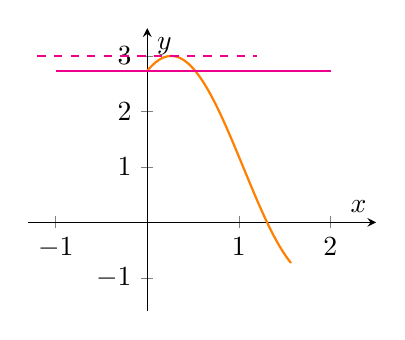
\begin{tikzpicture}[declare function={f(\k)=1+2*sin(deg(2*\k+pi/3));}]
          \tikzset{elegant/.style={smooth,thick,samples=50,magenta}}
          \begin{axis}[axis x line=middle,
                 axis y line=middle,
                 xmin=-1.3,xmax=2.5,
                 ymin=-1.6,ymax=3.5,
                 xstep=1,ystep=1,
                 ytick distance=1,
                 ylabel=$y$,
                 xlabel=$x$]
                \addplot[elegant,orange,domain=0:pi/2]{f(x)};
                \addplot[elegant,dashed,domain=-1.2:1.2]{3};
                \addplot[elegant,domain=-1:2]{2.732};
          \end{axis}
        \end{tikzpicture}
        当${x\in\Bigl[0,\dfrac{\piup}2\Bigr]}$时,$2x+\dfrac{\piup}3\in\Bigl[\dfrac{\piup}3,\dfrac{4\piup}3\Bigr]$,\\
        由图象得$f(0)=1+2\sin{\dfrac{\piup}3}=1+\sqrt3$,\\
        函数$f(x)$的最大值为$1+2=3$,\\
        $\therefore$要使方程$f(x)-m=2$在$x\in\Bigl[0,\dfrac{\piup}2\Bigr]$上有两个不同的解,
        则$f(x)=m+2$在$x\in\Bigl[0,\dfrac{\piup}2\Bigr]$上有两个不同的解,\\
        即函数$f(x)$和$y=m+2$在$x\in\Bigl[0,\dfrac{\piup}2\Bigr]$上有两个不同的交点,\\
        即$1+\sqrt3\leqslant m+2<3$,\\
        即 $\sqrt3-1\leqslant m<1$.
      \end{answer}
    \vspace{3.6cm}
    \item
      (本小题满分12分)\\
      已知向量$\bm a=\Bigl(\dfrac{1}2,\sin x\Bigr)$,$\bm b=\biggl(-1,\cos{\Bigl(x-\dfrac{\piup}6\Bigr)}\biggr)$,$f(x)=\bm a\cdot\bm b+\dfrac{1}4$,$(x\in\mathbb{R})$.\\
      (1)求函数$f(x)$的单调递减区间;\\
      (2)若函数$g(x)=f(x)-m,\Bigl(\dfrac{\piup}3\leqslant x\leqslant\dfrac{13\piup}{12}\Bigr)$有两个不同的零点$x_1,x_2$,求实数$m$的取值范围及$x_1,x_2$的和.\\
      \begin{answer}
        解:(1)$f(x)=\bm a\cdot\bm b+\dfrac{1}4
        =-\dfrac12+\sin{x}\cdot\cos{\Bigl(x-\dfrac{\piup}6\Bigr)}+\dfrac14
        =\sin{x}\cdot \Bigl(\cos x\cos{\dfrac{\piup}6}+\sin x\sin{\dfrac{\piup}6}\Bigr)-\dfrac14
        =\dfrac{\sqrt3}2\sin x\cos x+\dfrac12\sin^2x-\dfrac14
        =\dfrac{\sqrt3}4\sin{2x}-\dfrac14\cos{2x}
        =\dfrac12\sin{\Bigl(2x-\dfrac{\piup}6\Bigr)}$.\\
        由$2x-\dfrac{\piup}6\in\Bigl[\dfrac{\piup}2+2k\piup,\dfrac{3\piup}2+2k\piup\Bigr]$,${k\in\mathbb{Z}}$,解得$x\in\Bigl[\dfrac{\piup}3+k\piup,\dfrac{5\piup}6+k\piup\Bigr]$,${k\in\mathbb{Z}}$.\\
        $\therefore$函数$f(x)$的单调递减区间为$\Bigl[\dfrac{\piup}3+k\piup,\dfrac{5\piup}6+k\piup\Bigr]$,${k\in\mathbb{Z}}$.\\
        (2) $\because$函数$g(x)=f(x)-m,\Bigl(\dfrac{\piup}3\leqslant x\leqslant\dfrac{13\piup}{12}\Bigr)$有两个不同的零点$x_1,x_2$,
        $\therefore$函数$y=f(x)$的图像与函数$y=m$的图像在$\Bigl[\dfrac{\piup}3,\dfrac{13\piup}{12}\Bigr]$上有两个交点.\\
        又$\because \dfrac{\piup}3\leqslant x\leqslant\dfrac{13\piup}{12}$,
        $\therefore 2x-\dfrac{\piup}6\in\Bigl[\dfrac{\piup}2,2\piup\Bigr]$.
      \end{answer}
    \vspace{4cm}
    \item
      (本小题满分12分)\\
      如图,某污水处理厂要在一个矩形污水处理池($ABCD$)的池底水平铺设污水净化管道($Rt\triangle{FHE}$,$H$是直角顶点)米处理污水,管道越长,污水净化效果越好。设计要求管道的接口$H$是$AB$的中点,$E$、$F$分别落在线段$BC$、$AD$上.已知$AB=20$米,$AD=10\sqrt3$米,记$\angle{BHE}=\theta$.\\
      (1)试将污水净化管道的长度$l$表示为$\theta$的函数,并写出定义域;\\
      (2)若$\sin\theta+\cos\theta=\sqrt2$,求此时管道的长度$l$;\\
      (3)当$\theta$取何值时,污水净化效果好?并求出此时管道的长度.\\
      \begin{flushleft}
        \begin{tikzpicture}
          \coordinate[label=left:$A$](A)at(0,0);
          \coordinate[label=right:$B$](B)at(4,0);
          \coordinate[label=left:$D$](D)at(0,3.5);
          \coordinate[label=right:$C$](C)at(4,3.5);
          \draw[dashed] (A)rectangle(C);
          \coordinate[label=below:$H$](H)at(2,0);
          \coordinate[label=right:$E$](E)at(4,3);
          \path[name path=AD] (A)--(D);
          % \coordinate (P)at($(H)!2!90:(E)$);
          \path[name path=PH] ($(H)!1!90:(E)$)--(H);
          \path[name intersections={of=AD and PH}];
          \coordinate[label=left:$F$] (F)  at (intersection-1);
          % \draw[red] ($(H)!6pt!(E)$)--($(H)!6pt!(E)!6pt!90:(E)$)--($(H)!6pt!(F)$);
          \draw \rAm{E}{H}{F};
          % \draw [--] ($(H)+(0.5,0)$) arc (0:30:1cm);
          % \node at ($(H)+(0.8,0.3)$) {$\theta$};
          % \pic["\alpha",draw=red,angle radius=0.5cm] {angle=A--B--C};
          \path (B)--(H)--(E) pic [draw,"$\theta$",angle eccentricity=1.5] {angle=B--H--E};
          \draw (H)--(E)--(F)--cycle;
        \end{tikzpicture}
      \end{flushleft}
      \begin{answer}
        解:
      \end{answer}
    \vspace{1.5cm}
    \item%福州格致中学2015-2016学年高一数学第二学期期末检测.docx-22
      (附加题:本小题满分15分)\\
      (福州格致中学2015-2016学年高一数学第二学期期末检测22)已知函数$f(x)=A\sin(\omega x+\varphi)+B (A>0,\omega>0)$的一系列对应值如下表:
      \begin{center}
        \renewcommand{\arraystretch}{1.4}
        \begin{tabular}{|*{8}{c|}}
          \hline
            $x$
            &$-\dfrac{\piup}6$
            &$-\dfrac{\piup}3$
            &$-\dfrac{5\piup}6$
            &$-\dfrac{4\piup}3$
            &$-\dfrac{11\piup}6$
            &$-\dfrac{7\piup}3$
            &$-\dfrac{17\piup}6$\\
          \hline
            $y$
            &$-1$
            &$1$
            &$3$
            &$1$
            &$-1$
            &$1$
            &$3$\\
          \hline
        \end{tabular}\\
      \end{center}
      (1)根据表格提供的数据求函数$f(x)$的一个解析式;\\
      (2)根据(1)的结果:\\
      \;(i)当$x\in\Bigl[0,\dfrac{\piup}3\Bigr]$时,方程$f(3x)=m$恰有两个不同的解,求实数$m$的取值范围;\\
      \;(ii)若是$\alpha,\beta$是锐角三角形的两个内角,试比较$f(\sin \alpha)$与$f(\cos \beta)$的大小.
      \begin{answer}
        (1)$f(x)=2\sin\Bigl(x-\dfrac{\piup}3\Bigr)+1$;(2)(i)$[\sqrt{3}+1,3)$;(ii)易得$f(x)$在$[-\dfrac{\piup}6,\dfrac{5\piup}6]$上单调递增,故$f(x)$在$[0,1]$上单调递增;又$0<\dfrac{\piup}2-\beta<\alpha<\dfrac{\piup}2$,从而$\sin\alpha>\sin(\dfrac{\piup}2-\beta)=\cos\beta$,于是$f(\sin \alpha)>f(\cos \beta)$
      \end{answer}
    \vspace{4cm}
  \end{exercise}
  \stopexercise
\newpage
\centering{\heiti \xiaoer 福州清大教育2018-2019学年高一数学期末考模拟卷}\\
\part{\mbox{\heiti \xiaoer 参考答案}}
  \begin{multicols}{2}
    \printanswer
  \end{multicols}

% \Topic{函数的平移与伸缩变换&函数$y=A\sin (\omega x+\varphi)$的图像及简单应用}
  \Teach{函数$y=A\sin (\omega x+\varphi)$的图像变换}
  \Grade{高一}
  % \Name{郑皓天}\FirstTime{20181207}\CurrentTime{20181207}
  % \Name{林叶}\FirstTime{20180908}\CurrentTime{20181125}
  %\Name{1v2}\FirstTime{20181028}\CurrentTime{20181117}
  % \Name{林叶}\FirstTime{20180908}\CurrentTime{20181125}
  % \Name{郭文镔}\FirstTime{20181111}\CurrentTime{20181117}
  % \Name{马灿威}\FirstTime{20181111}\CurrentTime{20181111}
  \newtheorem*{Theorem}{定理}
  \makefront
\vspace{-1.5em}
\startexercise
\begin{exercise}{\heiti 课前检测}\\
\end{exercise}
\section{函数的(线性)变换}
  点$(x_0,y_0)$在图像$y=f(x)$上,则 $y_0=f(x_0)$\\
  点$(x_0-1,y_0)$在图像$y=f(x+1)$上\\
  点$(x_0,y_0-1)$在图像$y+1=f(x)$上\\
  点$(2x_0,y_0)$在图像$y=f(x/2)$上\\
  点$(x_0,2y_0)$在图像$y/2=f(x)$上\\
  点$(-x_0,y_0)$在图像$y=f(-x)$上\\
  点$(x_0,-y_0)$在图像$-y=f(x)$上\\
  当$\begin{cases}
      x_0=P(x')\\
      y_0=Q(y')
    \end{cases}$时,点$(x',y')$在图像$Q(y)=f(P(x))$上;也即\\
  在图像$Q(y)=f(P(x))$上每一点可由图像$y=f(x)$上的点$(x_0,y_0)$
  经变换$\begin{cases}
          x‘=P^{-1}(x_0)\\
          y’=Q^{-1}(y_0)
        \end{cases}$得到.
\section{函数$y=A\sin (\omega x+\varphi)$的图像}
  \begin{description}
    \item [label]
  \end{description}
  \begin{exercise}
    \qs
      函数$f(x)=\cos\left(\omega x+\varphi\right)$的部分图象如图所示,则$f(x)$的单调递减区间为\xx
      \begin{center}
      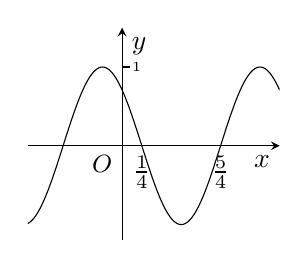
\begin{tikzpicture}
        \node[below left](O) at(0,0) {\small$\bm{O}$};
        \draw(0,1)node[right]{\tiny$1$}--(0.1,1);
        \clip(-1.2,-1.2) rectangle (2,1.5);
        \draw[->,>=stealth](-1.2,0)--(2,0) node[below left] (x){$x$};
        \draw[->,>=stealth](0,-1.2)--(0,1.5) node[below right] (y){$y$};
        \draw[domain=-1.2:2,samples=1000] plot(\x,{cos((pi*(\x)+1/4*pi) r)});
        \node[below] (A)at (0.25,0){$\frac{1}{4}$};
        \node[below] (B)at (1.25,0){$\frac{5}{4}$};
      \end{tikzpicture}
      \end{center}
      \twochx{$ \left(k\pi-\dfrac{1}{4},k\pi+\dfrac{3}{4}\right),k\inZ$}
        {$ \left(2k\pi-\dfrac{1}{4},2k\pi+\dfrac{3}{4}\right),k\inZ$}
        {$ \left(k-\dfrac{1}{4},k+\dfrac{3}{4}\right),k\inZ$}
        {$\left(2k-\dfrac{1}{4},2k+\dfrac{3}{4}\right),k\inZ $}
  \end{exercise}
\section{三角函数模型的简单应用-}
 \fz[12]
$f(x0)=d d$\fz[4]
\section{课后作业}
  \begin{exercise}

  \end{exercise}
\stopexercise
\section{参考答案}
\printanswer

% \Topic{三角函数单元复习}
  \Teach{}
  \Grade{高一}
  % \Name{郑皓天}\FirstTime{20181207}\CurrentTime{20181207}
  % \Name{林叶}\FirstTime{20180908}\CurrentTime{20181125}
  %\Name{1v2}\FirstTime{20181028}\CurrentTime{20181117}
  % \Name{林叶}\FirstTime{20180908}\CurrentTime{20181125}
  % \Name{郭文镔}\FirstTime{20181111}\CurrentTime{20181117}
  % \Name{马灿威}\FirstTime{20181111}\CurrentTime{20181111}
  \newtheorem*{Theorem}{定理}
  \makefront
\vspace{-1.5em}
\startexercise
% \begin{exercise}{\heiti 课前检测}\\
% \end{exercise}
\section{习题}
  % \begin{description}
  %   \item [label]
  % \end{description}
  \begin{exercise}
    \item%高中数学习题解法辞典.pdf 2-1-8
      已知$\abs{\cos \theta}\leqslant \abs{\sin\theta}$,则$\theta$的取值范围是\tk.
      \begin{answer}
        $\Bigl[k\piup+\dfrac{\piup}4,k\piup+\dfrac{3\piup}4\Bigr],k\in\mathbb{Z}$
      \end{answer}
    \item%高中数学习题解法辞典.pdf 2-1-19
      已知$\sin\Bigl(\dfrac{\piup}2+2x\Bigr)=-\dfrac12$,则$x=$\tk.
      \begin{answer}
        k\piup\pm\dfrac{\piup}3(k\in\mathbb{Z})
      \end{answer}
    \item%高中数学习题解法辞典.pdf 2-2-4
      函数$y=\sqrt{25-x^2}+\lg\sin\Bigl(x+\dfrac{\piup}3\Bigr)$的定义域为\tk.
      \begin{answer}
        $\Bigl[-5,-\dfrac{4\piup}3\Bigr)\bigcup\Bigl(-\dfrac{\piup}3,\dfrac{2\piup}3\Bigr)$
      \end{answer}
    \item%LaTeX-master/sanjiaohanshu/sanjiaohanshu-gaokao.tex 4
      函数$f(x)=\cos(\omega x+\varphi)$的部分图象如图所示,则$f(x)$的单调递减区间为\xz
      \begin{minipage}[b]{0.8\linewidth}
        \vspace{2.5em}
        \xx{$\Bigl(k\piup-\dfrac{1}{4},k\piup+\dfrac{3}{4}\Bigr),k\in\mathbb{Z}$}
          {$ \Bigl(2k\piup-\dfrac{1}{4},2k\piup+\dfrac{3}{4}\Bigr),k\in\mathbb{Z}$}
          {$ \Bigl(k-\dfrac{1}{4},k+\dfrac{3}{4}\Bigr),k\in\mathbb{Z}$}
          {$\Bigl(2k-\dfrac{1}{4},2k+\dfrac{3}{4}\Bigr),k\in\mathbb{Z} $}
      \end{minipage}\hfill
      \begin{minipage}[h]{0.2\linewidth}
        \vspace{-3cm}
        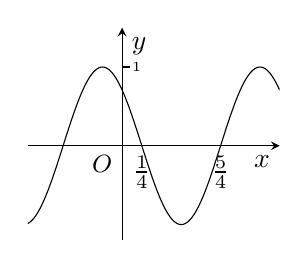
\begin{tikzpicture}
          \node[below left](O) at(0,0) {\small$\bm{O}$};
          \draw(0,1)node[right]{\tiny$1$}--(0.1,1);
          \clip(-1.2,-1.2) rectangle (2,1.5);
          \draw[->,>=stealth](-1.2,0)--(2,0) node[below left] (x){$x$};
          \draw[->,>=stealth](0,-1.2)--(0,1.5) node[below right] (y){$y$};
          \draw[domain=-1.2:2,samples=1000] plot(\x,{cos((pi*(\x)+1/4*pi) r)});
          \node[below] (A)at (0.25,0){$\frac{1}{4}$};
          \node[below] (B)at (1.25,0){$\frac{5}{4}$};
        \end{tikzpicture}
      \end{minipage}
      \begin{answer}
        D
      \end{answer}
    \item%《习题化知识清单》P72知识2-2
      不等式$\tan x>a$在$x\in\Bigl(-\dfrac{\piup}4,\dfrac{\piup}2 \Bigr)$上恒成立,则$a$的取值范围是\xz
      \xx{$(-\infty,-1]$}
        {$(-\infty,-1)$}
        {$(-\infty,1]$}
        {$(-\infty,1]$}
      \begin{answer}
        A
      \end{answer}
    \item%福州三中中学2015-2016学年高一数学第二学期期末检测.docx-9
      (福州三中中学2015-2016学年高一数学第二学期期末检测9)将函数$y=\sin\Bigl(x-\dfrac{\piup}3\Bigr)$的图像上所有点的横坐标伸长到原来的2倍(纵坐标不变),再将所得的图像向左平移$\dfrac{\piup}3$个单位,得到的函数图像对应的解析式是\xz
      \xx{$y=\sin\dfrac x2$}
        {$y=\sin\Bigl(\dfrac x2-\dfrac{\piup}2\Bigr)$}
        {$y=\sin\Bigl(\dfrac{x}2-\dfrac{\piup}6\Bigr)$}
        {$y=\sin\Bigl(2x-\dfrac{\piup}6\Bigr)$}
      \begin{answer}
        C
      \end{answer}
    \item%《习题化知识清单》P73易混清单例
      函数$y=2\sin\Bigl(\dfrac{\piup}3-2x \Bigr)$的单调增区间为\tk.
      \begin{answer}
        $\Bigl[k\piup+\dfrac{5\piup}{12},k\piup+\dfrac{11\piup}{12} \Bigr],k\in\mathbb{Z}$
      \end{answer}
    \item%《习题化知识清单》P72例1
      函数$\dfrac{\sin x+2}{\sin x+1},x\in\Bigl[0,\dfrac{\piup}2\Bigr]$的值域为\tk.
      \begin{answer}
        $\Bigl[\dfrac32,2\Bigr]$
      \end{answer}
    \item%LaTeX-master/sanjiaohanshu/gaokaosection.tex 31
      把函数$ y=\sin 2x $的图象沿$x$轴向左平移$ \dfrac{\piup}{6} $个单位,纵坐标伸长到原来的2倍(横坐标不变)后得到函数$ y=f(x) $的图象,对于函数$ y=f(x) $有以下四个判断:\\
      \ding{192} 该函数的解析式为$ y=2\sin \Bigl(2x+\dfrac{\piup}{6}\Bigr) $;\\
      \ding{193} 该函数图象关于点$ \Bigl(\dfrac{\piup}{3},0\Bigr) $对称;\\
      \ding{194} 该函数在$ \Bigl[0,\dfrac{\piup}{6}\Bigr] $上是增函数;\\
      \ding{195} 若函数$ y=f(x)+a $在$ \Bigl[0,\dfrac{\piup}{2}\Bigr] $上的最小值为$ \sqrt{3},\  $则$ a=2\sqrt{3} .$\\
      其中,正确判断的序号是\tk.
      \begin{answer}
        \circled{2}\circled{4}
      \end{answer}
    \item%福州格致中学2015-2016学年高一数学第二学期期末检测.docx-22
      (福州格致中学2015-2016学年高一数学第二学期期末检测22)已知函数$f(x)=A\sin(\omega x+\varphi)+B (A>0,\omega>0)$的一系列对应值如下表:
      \begin{center}
        \renewcommand{\arraystretch}{1.4}
        \begin{tabular}{|*{8}{c|}}
          \hline
            $x$
            &$-\dfrac{\piup}6$
            &$-\dfrac{\piup}3$
            &$-\dfrac{5\piup}6$
            &$-\dfrac{4\piup}3$
            &$-\dfrac{11\piup}6$
            &$-\dfrac{7\piup}3$
            &$-\dfrac{17\piup}6$\\
          \hline
            $y$
            &$-1$
            &$1$
            &$3$
            &$1$
            &$-1$
            &$1$
            &$3$\\
          \hline
        \end{tabular}\\
      \end{center}
      (1)根据表格提供的数据求函数$f(x)$的一个解析式;\\
      (2)根据(1)的结果:\\
      \;(i)当$x\in\Bigl[0,\dfrac{\piup}3\Bigr]$时,方程$f(3x)=m$恰有两个不同的解,求实数$m$的取值范围;\\
      \;(ii)若是$\alpha,\beta$是锐角三角形的两个内角,试比较$f(\sin \alpha)$与$f(\cos \beta)$的大小.
      \begin{answer}
        (1)$f(x)=2\sin\Bigl(x-\dfrac{\piup}3\Bigr)+1$;(2)(i)$[\sqrt{3}+1,3)$;(ii)易得$f(x)$在$[-\dfrac{\piup}6,\dfrac{5\piup}6]$上单调递增,故$f(x)$在$[0,1]$上单调递增;又$0<\dfrac{\piup}2-\beta<\alpha<\dfrac{\piup}2$,从而$\sin\alpha>\sin(\dfrac{\piup}2-\beta)=\cos\beta$,于是$f(\sin \alpha)>f(\cos \beta)$
      \end{answer}
    \vspace{6.5cm}
    \item%高中数学习题解法辞典.pdf 2-2-9
      已知函数$y=f(x)$的定义域为$\mathbb{R}$,若$f(x+2)=-f(x)$,且当$-1\leqslant x\leqslant 1$时,$f(x)=x$,求证:\\
      (1)函数$y=f(x)$是最小正周期为4的周期函数;\\
      (2)函数$y=f(x)$是奇函数;\\
      (3)当$x\in[4k-1,4k+1](k\in\mathbb{Z})$时,$y=f(x)$是增函数;当$x\in[4k+1,4k+3](k\in\mathbb{Z})$时,$y=f(x)$是减函数.
      % \begin{answer}
      %
      % \end{answer}
  \end{exercise}

\newpage
\section{课后作业}
  \begin{exercise}
    \item%高中数学习题解法辞典.pdf 2-1-74
      已知$1+\sin^2x=\cos x$,则$x=$\tk.
      \begin{answer}
        $2k\piup(k\in\mathbb{Z})$
      \end{answer}
    \item%《习题化知识清单》P72方法2-1
      函数$\abs{\sin x}$的一个单调区间是\xz
      \xx{$\Bigl(\dfrac{\piup}2,\piup\Bigr)$}
        {$\Bigl(\piup,2\piup\Bigr)$}
        {$\Bigl(\piup,\dfrac{3\piup}2\Bigr)$}
        {$\Bigl(0,\piup\Bigr)$}
      \begin{answer}
        C
      \end{answer}
    \item%LaTeX-master/sanjiaohanshu/gaokaosection.tex 13
       已知函数$f(x)=\Bigg\{\begin{aligned}
      \sin(x+a),x\le 0\\\cos (x+b),x>0
      \end{aligned}$是偶函数,则下列结论可能成立的是\xz
       \xx{$ a=\dfrac{\piup}{4},b=-\dfrac{\piup}{4}$}
        {$ a=\dfrac{2\piup}{3},b=\dfrac{\piup}{6}$}
        {$a=\dfrac{\piup}{3},b=\dfrac{\piup}{6} $}
        {$ a=\dfrac{5\piup}{6},b=\dfrac{2\piup}{3}$}
      \begin{answer}
        C
      \end{answer}
    \item%《习题化知识清单》P77单元检测10
      定义在$\mathbb{R}$上的偶函数$f(x)$满足$f(x+1)=-\dfrac2{f(x)}(f(x)\neq0)$,且在区间$(2013,2014)$上单调递增.已知$\alpha,\beta$是锐角三角形的两个内角,则$f(\sin\alpha),f(\cos\beta)$的大小关系是\xz
      \xx{$f(\sin\alpha)<f(\cos\beta)$}
        {$f(\sin\alpha)>f(\cos\beta)$}
        {$f(\sin\alpha)=f(\cos\beta)$}
        {以上情况均有可能}
    \item%《习题化知识清单》P72知识3-3
      若函数$y=2\cos(2x+\varphi)$是偶函数,且在$\Bigl(0,\dfrac{\piup}4\Bigr)$上是增函数,则实数$\varphi$可能是\xz
      \xx{$-\dfrac{\piup}2$}
        {0}
        {{$\dfrac{\piup}2$}}
        {$\piup$}
      \begin{answer}
        D
      \end{answer}
    \item%高中数学习题解法辞典.pdf 2-1-74
      比较$\sin 3$,$\cos 3$,$\tan 0.8$的大小关系为\tk.
      \begin{answer}
        $\tan 0.8>\sin 3>\cos 3$
      \end{answer}
    \item%LaTeX-master/sanjiaohanshu/gaokaosection.tex 26
      已知函数$f(x)=\sin (2x+\varphi)$,若$    f\Bigl(\dfrac{\piup}{12}\Bigr)-f\Bigl(-\dfrac{5\piup}{12}\Bigr)=2 $,则函数$f(x)$的单调增区间为\tk.
      \begin{answer}
        $\Bigl[k\piup-\dfrac{5\piup}{12},k\piup+\dfrac{\piup}{12}\Bigr],k\in\mathbb{Z}$
      \end{answer}
    \item%函数y=Asin(ωx+φ)的图象及简单应用P11.9
      若$f(x)=\cos\Bigl(2x+\dfrac{\piup}3+\varphi\Bigr)$$(\abs{\varphi}<\dfrac{\piup}2)$是奇函数,则$\varphi=$\tk.
      \begin{answer}
        $\dfrac{\piup}6$
      \end{answer}
    \item%《习题化知识清单》P77单元检测12
      设$\omega>0$,若函数$f(x)=2\sin \omega x(\omega>0)$在区间$\Bigl[-\dfrac{\piup}3,\dfrac{\piup}4 \Bigr]$上单调递增,则$\omega$取值范围是\tk.
      \begin{answer}
        $\Bigl(0,\dfrac32\Bigr]$
      \end{answer}
    \item%高中数学习题解法辞典.pdf 2-2-1
      已知函数$f(x)=A\sin(\omega x+\varphi)(A,\omega,\varphi\text{为常数},\omega>0)$的图像上相邻两个最高点的坐标分别是$\Bigl(\dfrac{\piup}{12},2\Bigr)$,$\Bigl(\dfrac{13\piup}{12},2\Bigr)$.\\
      (1) 求函数$f(x)$的一个表达式;\\
      (2)画出函数$f(x)$在长度为一个周期的闭区间上的简图;\\
      (3)说明经过怎样的变换,可以由$y=\sin x$的图像得到$y=f(x)$的图像.
      \begin{answer}
        (1)$y=2\sin\Bigl(2x+\dfrac{\piup}3\Bigr)(\varphi=k\piup-\dfrac{2\piup}3$即可);(2)略;(3)将$y=\sin x$图像上所有点向左平移$\dfrac{\piup}3$个单位得到$y=\sin \Bigl(x+\dfrac{\piup}3\Bigr)$的图像;再把$y=\sin \Bigl(x+\dfrac{\piup}3\Bigr)$的图像上所有点的横坐标缩短到原来的$\dfrac12$(纵坐标不变),得到$y=\sin \Bigl(2x+\dfrac{\piup}3\Bigr)$的图像;最后把$y=\sin \Bigl(2x+\dfrac{\piup}3\Bigr)$的图像上所有点的纵坐标伸长到原来的2倍(横坐标不变),即可得到函数$y=f(x)$的图像.
      \end{answer}
    \vspace{6cm}
    \item%函数y=Asin(ωx+φ)的图象及简单应用P11.14
      已知曲线$y=A\sin(\omega x+\varphi)$$(A>0,\omega>0,\abs{\varphi}\leqslant\dfrac{\piup}2)$上最高点为$(2,\sqrt{2})$,该最高点与相邻的最低点间的曲线与$x$轴交于点$(6,0)$.\\
      (1)该函数的解析式;\\
      (2)该函数在$x\in[-6,0]$上的值域.
      \begin{answer}
        (1)$y=\sqrt{2}\sin\Bigl(\dfrac{\piup}8x+\dfrac{\piup}4\Bigr)$;
        (2)$[-\sqrt{2},0]$
      \end{answer}
    \vspace{5cm}
    \item%高中数学习题解法辞典.pdf 2-2-44
      已知函数$f(x)=2\sin\Bigl(\omega x+\dfrac{\piup}6\Bigr)(\omega>0)$,\\
      (1)求$f(x)$的最大值$M$,最小值$m$以及最小正周期$T$;\\
      (2)试求最小正整数$\omega$,使得自变量$x$在任意两个整数间(包括整数本身)变化时,函数$f(x)$至少有一个值是$M$,另一个值是$m$.
      \begin{answer}
        (1)$M=3,m=-1,T=\dfrac{2\piup}{\omega}$;(2)$\dfrac{2\piup}{\omega}\leqslant 1$,$\omega=7$
      \end{answer}
    \vspace{6cm}
    \item%高中数学习题解法辞典.pdf 2-2-45
      求证:(1)$f(x)=\sin x\cos x$的最小正周期为$\piup$;\\
      (2)若函数$y=f(x)(x\in\mathbb{R})$的最小正周期为$T$,则$f(kx)(k>0)$的最小正周期为$\dfrac{T}k$.
      \begin{answer}
        (1)(提示:若$0<T<\piup$,令$x=0$,得$T=\dfrac{\piup}2$,不符);(2)(提示:$f\biggl[k\Bigl(x+\dfrac{T}k\Bigr)\biggr]=f(kx+T)=f(kx)$)
      \end{answer}
  \end{exercise}
\stopexercise

\newpage
\section{部分参考答案}
\begin{multicols}{2}
  \printanswer
\end{multicols}

% \input{b5.2.1-vector.tex}
% \Topic{平面向量坐标表示,数量积}
  \Teach{向量共线与数量积的坐标表示}
  \Grade{高一}
  % \Name{郑皓天}\FirstTime{20181207}\CurrentTime{20181207}
  % \Name{林叶}\FirstTime{20180908}\CurrentTime{20181125}
  % \Name{1v2}\FirstTime{20181028}\CurrentTime{20181117}
  % \Name{林叶}\FirstTime{20180908}\CurrentTime{20181125}
  % \Name{郭文镔}\FirstTime{20181111}\CurrentTime{20181117}
  % \Name{马灿威}\FirstTime{20181111}\CurrentTime{20181111}
  \newtheorem*{Theorem}{定理}
  \makefront
\vspace{-1.5em}

\startexercise
% \begin{exercise}{\heiti 课前检测}\\
%   表格实例:
%   \begin{center}
%     \renewcommand{\arraystretch}{1.4}
%     \begin{tabular}{|*{8}{c|}}
%       \hline
%         $x$
%         &$-\dfrac{\piup}6$
%         &$-\dfrac{\piup}3$
%         &$-\dfrac{5\piup}6$
%         &$-\dfrac{4\piup}3$
%         &$-\dfrac{11\piup}6$
%         &$-\dfrac{7\piup}3$
%         &$-\dfrac{17\piup}6$\\
%       \hline
%         $y$
%         &$-1$
%         &$1$
%         &$3$
%         &$1$
%         &$-1$
%         &$1$
%         &$3$\\
%       \hline
%     \end{tabular}\\
%   \end{center}
% \end{exercise}

\section{平面向量基本定理及坐标表示}
  \subsection{基底}
    \begin{Theorem}[平面向量基本定理]
      如果$ \bm{e}_1,\bm{e}_2 $是同一平面内的两个\CJKunderdot{不共线}的向量,那么对于这一平面内的任意向量$ \bm{a} $,有且只有一对实数$ \lambda_1,~\lambda_2 $,使$\bm{a}=\lambda_1\bm{e}_1+\lambda_2\bm{e}_2$.\par 其中,不共线的向量$ \bm{e}_1,~\bm{e}_2 $叫做表示这一平面内所有向量的一组\CJKunderdot{基底}.
    \end{Theroem}
    {\kaishu 解决向量问题,需要注意两点:一是向量共线定理,一个是平面向量基本定理.\par
    向量的基底的重要性在于一旦有了基底,你就可以将题目中涉及的所有向量都用基底向量唯一的表示出来(坐标表示就是一组特殊的基底),计算和变形都有了方向,便于寻找和发现关系.如果题目没有明确给出基底,那么就需要自己指定了}
  \subsection{坐标表示}
    在不共线的向量中,垂直是一种重要的情形,把一个向量分解为两个互相垂直的向量,叫做把向量\CJKunderdot{正交分解}.\par
    在平面直角坐标系$xOy$中,分别取与$x$轴、$y$轴方向相同的两个\CJKunderdot{单位向量}$~ \bm{i},~\bm{j} $作为基底.对于平面内的一个向量$ \bm{a} $,由平面向量基本定理可知,有且只有一对实数$ x,~y $使得\[\bm{a}=x\bm{i}+y\bm{j}\]
    这样,平面内的任一向量$ \bm{a} $都可以由$ x,~y $唯一确定,我们把有序数对$ (x,y) $叫做向量$\bm{a}  $的坐标,记作
    \begin{equation}\label{eq:axy}
      \bm{a}=(x,y)
    \end{equation}
    其中$ x $叫做$ \bm{a} $在$x$轴上的坐标,$ y $叫做$ \bm{a} $在$y$轴上的坐标,(\ref{eq:axy})式叫做\textbf{向量的坐标表示}
    \begin{center}
    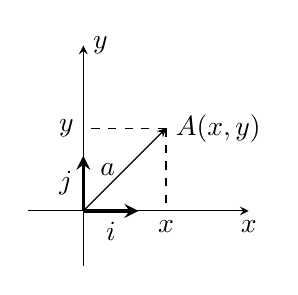
\begin{tikzpicture}[scale=0.7]
      \draw[->,>=stealth] (-1,0)--(3,0) node[below](x){$x$};
      \draw[->,>=stealth] (0,-1)--(0,3) node[right](y){$y$};
      \draw[very thick,->,>=stealth](0,0)--(1,0)node[midway,below](i) {$\bm{i}$};
      \draw[very thick,->,>=stealth](0,0)--(0,1)node[midway,left](j) {$\bm{j}$};
      \coordinate(A) at (1.5,1.5);
      \node[right](a1)at(1.5,1.5){$A(x,y)$};
      \draw[dashed](A)--++(-1.5,0)node[left](y){$y$};
      \draw[dashed](A)--++(0,-1.5)node[below](x){$x$};
      \draw[->,>=stealth](0,0)--(A) node[midway,left] (a) {$\bm{a}$};
    \end{tikzpicture}
    \end{center}
    \begin{description}
      \item[三点共线的判定] 若$ A,~B,~C $三点共线,有$ \vv{OA}=\lambda \vv{OB}+\mu\vv{OC}~(\lambda+\mu=1) $.或$\vv{AB}=\lambda \vv{AC}$.
      %\begin{enumerate}[1)]
      %
      %\end{enumerate}
    \end{description}
  \subsection{平面向量的坐标计算}
    \begin{enumerate}
      \item
        设点$ A(x_1,y_1),~B(x_2,y_2) $,则$ \vv{AB}=(x_2-x_1,y_2-y_1) $.\par
        一个向量的坐标等于表示此向量的有向线段的终点的坐标减去起始点的坐标.
      \item
        若$\bm{a}=\left(x_1,y_1\right),\bm{b}=\left(x_2,y_2\right)$.
        \begin{description}
          \item[加法:]
            $\bm{a}+\bm{b}=(x_1+x_2,y_1+y_2)$
            \begin{equation*}
            \begin{aligned}
            \bm{a}+\bm{b}=&\left(x_1\bm{i}+y_1\bm{j}\right)+\left(x_2\bm{i}+y_2\bm{j}\right)\\
            =&\left(x_1+x_2\right)\bm{i}+\left(y_1+y_2\right)\bm{j}\\
            \text{即:}\bm{a}+\bm{b}=&(x_1+x_2,y_1+y_2)
            \end{aligned}
            \end{equation*}
          \item[减法:] $\bm{a}-\bm{b}=\left(x_1-x_2,y_1-y_2\right)$.同加法可得
          \item[数乘:]
            $ \lambda \bm{a}=\left(\lambda x_1,\lambda y_1\right) $\begin{equation*}
            \begin{aligned}
             \lambda \bm{a} =&\lambda\left(x_1\bm{i}+y_1\bm{j}\right)=\lambda x_1\bm{i}+\lambda y_1\bm{j}\\
            =&\left(\lambda x_1,\lambda y_1\right)
            \end{aligned}
            \end{equation*}
          \item[模长]
           $\abs{\bm{a}}=\sqrt{x_1^2+y_1^2}$\qquad
           $\abs{\vv{AB}}=\sqrt{(x_2-x_1)^2+(y_2-y_1)^2}$\\
           \qquad $\abs{\bm{a}+\bm{b}}=\sqrt{(\bm{a}+\bm{b})^2}=\sqrt{\bm{a}^2+2\bm{a}\bm{\cdot}\bm{b}+\bm{b}^2}$\\
          \item[共线]$\bm{a} \varparallel \bm{b}\Leftrightarrow x_1y_2=y_2x_1 $\\
            由向量共线的性质知$ \bm{a} $与$ \bm{b}(\bm{b}\ne\bm{0}) $共线,当且仅当存在实数$ \lambda $使得$ \bm{a}=\lambda \bm{b} .$\\用坐标表示为:
            $$(x_1,y_1)=\lambda(x_2,y_2)$$
            即$$\Bigg\{\begin{aligned}
            x_1=&\lambda x_2\\
            y_1=&\lambda y_2
            \end{aligned}$$
            消去$ \lambda $得到\[x_1y_2-x_2y_1=0\]
          \item[垂直]
            $\bm{a}\perp\bm{b}\Leftrightarrow\bm{a}\bm{\cdot}\bm{b}=0\Leftrightarrow x_1x_2+y_1y_2=0 $
            \begin{proof}
              \begin{description}
                \item[方法一]
                  设$ \bm{a},~\bm{b} $所在直线分别为$ l_1,l_2 $,当$ \bm{a},~\bm{b} $所在直线的斜率都存在时,由直线垂直的性质,有$$ k_{l_1}\bm{\cdot}k_{l_2}=-1 $$
                  其中$$ k_{l_1} =\dfrac{y_1-0}{x_1-0}=\dfrac{y_1}{x_1},\quad k_{l_2} =\dfrac{y_2-0}{x_2-0}=\dfrac{y_2}{x_2}$$
                  即$$\dfrac{y_1}{x_1}\bm{\cdot}\dfrac{y_2}{x_2}=-1$$
                  $$x_1x_2+y_1y_2=0$$
                \item[方法二]
                  由向量的数量积性质,当$ \bm{a}\perp\bm{b} $时,
                  $\text{由}\cos\theta=\dfrac{\bm{a\cdot b}}{\abs{\bm{a}}\abs{\bm{b}}}\text{得到}$\\
                  \centering $\bm{a\cdot b}=0$
              \end{description}
            \end{proof}
        \end{description}
    \end{enumerate}
  \begin{exercise}{{\textbf{基础练习}}}
    \item%《习题化知识清单》P82知识1-3【平面向量基本定理】
      已知向量$\bm a=(1,2)$,$\bm b=(-2,3)$,$\bm c=(4,1)$,若用$\bm a$和$\bm b$表示$\bm c$,则$\bm c=$\tk.
      \begin{answer}
        $2\bm a-\bm b$
      \end{answer}
    \item%《习题化知识清单》P82知识2-1【向量坐标运算】
      设平面向量$\bm a=(3,5)$,$\bm b=(-2,1)$,则$\bm a-2\bm b=$\xz
      \xx{(7,3)}{(7,7)}{(1,7)}{(1,3)}
      \begin{answer}
        A
      \end{answer}
    \item%《习题化知识清单》P82知识2-2【向量坐标运算,单位向量】
      已知$\bm a=(3,4)$,则与$\bm a$同向的单位向量的坐标是\xz
      \xx{$(3,4)$}
       {$(-\dfrac{3}5,\dfrac{4}5)$}
       {$(-\dfrac{3}5,-\dfrac{4}5)$}
       {$(\dfrac{3}5,\dfrac{4}5)$}
      \begin{answer}
        D
      \end{answer}
    \item%《习题化知识清单》P82知识2-3【向量坐标运算,中点坐标公式】
      已知平面直角坐标系$xOy$内的三点分别是$A(2,-5)$,$B(3,4)$,$C(-1,-3)$,$D$为线段$BC$的中点,则向量$\vv{DA}$的坐标为\tk.
    \item%《习题化知识清单》P82知识3-1【向量共线】
      设向量$\bm a=(m,1)$,$\bm b=(1,m)$,如果$\bm a$与$\bm b$共线且方向相反,那么$m$的值为\xz
      \xx{$1$}{$-1$}{$\pm 1$}{$0$}
      \begin{answer}
        B
      \end{answer}
    \item%《习题化知识清单》P82知识3-3【向量共线,三角函数的定义】
      若$\bm a=\Bigl(\dfrac{3}2,\sin\alpha\Bigr)$,$\bm b=\Bigl(\sin\alpha,\dfrac{1}3\Bigr)$,且$\bm a\varparallel \bm b$,则锐角$\alpha$为\xz
      \xx{30\degree}{45\degree}{60\degree}{75\degree}
      \begin{answer}
        B
      \end{answer}
    \item%《习题化知识清单》P82知识3-4【向量共线坐标表示】
      若向量$\vv{OA}=(k,6)$,$\vv{OB}=(4,5)$,$\vv{OC}=(1-k,10)$,且$A$,$B$,$C$三点共线,则$k=$\tk.
      \begin{answer}
        $\dfrac{17}6$
      \end{answer}
  \end{exercise}
\section{平面向量的数量积}
  \subsection{定义}
    \begin{description}
      \item[定义] 已知两个非零向量$ \bm{a} $与$\bm{b}$,我们把数量$ \abs{\bm{a}}\abs{\bm{b}}\cos\theta $叫做$ \bm{a} $与$ \bm{b} $的\textbf{数量积}(又称点积、内积),记作$ \bm{a}\bm{\cdot}\bm{b} $,即\[\bm{a}\bm{\cdot}\bm{b}=\abs{\bm{a}}\abs{\bm{b}}\cos\theta\]
      其中$ \theta $为$ \bm{a} $与$ \bm{b} $的夹角.\\
      $\abs{\bm{a}}\cos\theta$($\abs{\bm{b}}\cos\theta$)叫做向量$\bm a$在$\bm b$方向上($\bm b$在$\bm a$方向上)的\textbf{投影},记作$\mathrm{Prj}_{\bm b}{\bm a}$(或$\mathrm{Prj}_{\bm b}{\bm a}$)
      \item[几何意义] 两个向量的数量积等于其中一个向量的模长与另一个向量在此向量方向上的投影的乘积%$ \bm{a}\bm{\cdot}\bm{b} $等于$\bm{a} $的模长$ \abs{\bm{a}} $与$ \bm{b} $在$ \bm{a} $的方向上的\textbf{投影}$ \abs{\bm{b}}\cos \theta $的乘积.\par
      {\kaishu \textbf{注:}当$ \theta=0 $时,$ \cos\theta=1 $,所以有$ \bm{a\cdot b}=\bm{\abs{a}\abs{b}} $;\\\phantom{注:\ }当$ \theta=90^{\circ} $时,有$ \cos\theta =0$,所以有$ \bm{a\cdot b}=0 $ \\\phantom{注:\ }当$ \theta=180^{\circ} $时,有$ \cos\theta =-1$,所以有$ \bm{a\cdot b}=\abs{\bm{a}}\abs{\bm{b}} $   }
      \item[数量积计算]
      \begin{equation*}
      \begin{aligned}
      &\because \bm{a}=x_1\bm{i}+y_1\bm{j},~\bm{b}=x_2\bm{i}+y_2\bm{j},\\
      &\therefore \bm{a}\bm{\cdot}\bm{b}=(x_1\bm{i}+y_1\bm{j})\bm{\cdot}(x_2\bm{i}+y_2\bm{j})\\
      &\phantom{\therefore\bm{a}\bm{\cdot}\bm{b}~}=x_1x_2\bm{i}^2+x_1y_2\bm{i}\bm{\cdot}\bm{j}+x_2y_1\bm{i}\bm{\cdot}\bm{j}+y_1y_2\bm{j}^2.\\
      & \bm{i}^2=\bm{j}^2=1,\bm{i}\bm{\cdot}\bm{j}=\bm{j}\bm{\cdot}\bm{i}=0\\
      &\therefore \bm{a}\bm{\cdot}\bm{b}=x_1x_2+y_1y_2.
      \end{aligned}
      \end{equation*}
      \item[运算律]已知向量$\bm a$,$\bm b$,$\bm c$和实数$\lambda$,则:
        \begin{itemize}%[leftmargin=*]
          \item 交换律:$\bm{a}\cdot\bm{b}=\bm{b}\cdot\bm{a}$;
          \item 分配律:$(\bm a+\bm b)\cdot \bm c=\bm a\cdot\bm c+\bm b\cdot \bm c$;
          \item $(\lambda \bm a)\cdot\bm{b}=\lambda(\bm a\cdot\bm b)=\bm{a}\cdot(\lambda\bm{b})$.
        \end{itemize}
      \item[夹角公式] \[ \cos\theta=\dfrac{\bm{a}\bm{\cdot}\bm{b}}{\abs{\bm{a}}\abs{\bm{b}}}=\dfrac{x_1x_2+y_1y_2}{\sqrt{x_1^2+y_1^2}\sqrt{x_2^2+y_2^2}} \quad \left(\theta\in\left[0,\pi\right],~\theta\text{也写作}\left<\bm{a},\bm{b}\right>\right).\]
    \end{description}\par
    {\kaishu 直接求向量的数量积的方是近年高考的重点,其关键是根据向量的加减法则对向量进行基底分解.分解以后可以直接使用题目的已知条件,要么出现所要求的表达式(此时通过解一元一次方程).分解过程中,往往利用\CJKunderdot{垂直}将数量积消掉.\CJKunderdot{整体}的思想在数学中占据着极其重要的位置,求解整体的值时,往往不需要分别求出各个元素的值,而是将元素进行有效的分解、整合,提取有效的信息,从而求出整体的值.}
    %\subsection{求向量夹角的方法}
    %\begin{description}
    %\item[坐标法] $\cos\theta=\dfrac{x_1x_2+y_1y_2}{\sqrt{x_1^2+y_1^2}\sqrt{x_2^2+y_2^2}}$
    %\item[向量法] $\cos\theta=\dfrac{\bm{a}\bm{\cdot}\bm{b}}{\abs{\bm{a}}\abs{\bm{b}}}$
    %\end{description}
  \subsection{数量积相关补充}
    \begin{enumerate}[label=\circled{\arabic*}]
      \item 若$\bm{a}=\left(x,y\right)$,则$ \bm{a}\bm{\cdot}\bm{a}=\bm{a}^2=\abs{\bm{a}}^2=x^2+y^2 $;
      \item $ \left(\bm{a}\pm \bm{b}\right)^2=\abs{\bm{a}\pm \bm{b}}^2=\abs{\bm a}^2\pm2\bm{a}\bm{\cdot}\bm{b}+\abs{\bm b}^2=\bm{a}^2\pm2\bm{a}\bm{\cdot}\bm{b}+\bm{b}^2$;
      \item $\bm a^2-\bm b^2=(\bm a+\bm b)\cdot(\bm a-\bm b)=\abs{\bm a}^2-\abs{\bm b}^2$;
      \item $\bm a^2+\bm b^2=0\Leftrightarrow \bm a=\bm b=0$
      \item $\bigm|\abs{\bm{a}}-\abs{\bm{b}}\bigm|\le\abs{\bm{a\pm b}}\le\abs{\bm{a}}+\abs{\bm{b}}$;
      \item 若点$ A(x_1,y_1),~B(x_2,y_2) $,则$ \abs{\vv{AB}}=\sqrt{(x_2-x_1)^2+(y_2-y_1)^2} $;
      \item \textbf{柯西-施瓦兹不等式:}若$\bm{a}=\left(x_1,y_1\right),\bm{b}=\left(x_2,y_2\right)$,则:$$ -\abs{\bm{a}}\abs{\bm{b}}\le\bm{a}\bm{\cdot}\bm{b}\le\abs{\bm{a}}\abs{\bm{b}}\Leftrightarrow -\sqrt{x_1^2+y_1^2}\sqrt{x_2^2+y_2^2}\le x_1x_2+y_1y_2\le \sqrt{x_1^2+y_1^2}\sqrt{x_2^2+y_2^2}$$
      \item 若$ \abs{\bm{a}+\bm{b}}=\abs{\bm{a}-\bm{b}} $,则$ \bm{a}\perp\bm{b} $.对角线相等的平行四边形必然是矩形.
      \item 若$ \left(\bm{a}+\bm{b}\right)\perp\left(\bm{a}-\bm{b}\right) $,则$\abs{\bm{a}}=\abs{\bm{b}} $.对角线垂直的平行四边形必然是菱形.
      \item 平面上$ O,~A,~B $三点不共线,设$\vv{OA}=\bm{a}=(x_1,y_1) ,~\vv{OB}=\bm{b}=(x_2,y_2)$,则$$ S_{\triangle OAB}=\dfrac{1}{2}\sqrt{\abs{\bm{a}}^2\abs{\bm{b}}^2-\left(\bm{a}\bm{\cdot}\bm{b}\right)^2}=\dfrac{1}{2}\abs{x_1y_2-x_2y_1} .$$
      \item 给定两个长度为$ a $的平面向量$ \vv{OA},~\vv{OB} $,其夹角为$ \theta\in\left[0,\pi \right), ~$点$ C $在以$ O $为圆心的圆弧$ AB $上变动,若$ \vv{OC}=x\vv{OA}+y\vv{OB},~x,y\inR $,则$ x+y $的最大值为$ \sqrt{\dfrac{2}{\cos\theta+1}}. $
    \end{enumerate}
  \begin{exercise}{{\textbf{基础练习}}}
    \item%《习题化知识清单》P83知识1-1【数量积的定义、性质】
      在$\triangle{ABC}$中,$AB=BC=2$,$\angle{B}=\dfrac{\piup}4$,$AD$是边$BC$上的高,则$\vv{AD}\cdot\vv{AC}$的值为\xz
      \xx{0}{2}{4}{8}
      \begin{answer}
        B
      \end{answer}
    \item%《习题化知识清单》P83知识1-2【数量积的定义、性质】
      已知$\triangle{ABC}$中,$AB=AC=BC=6$,平面内一点$M$满足$\vv{BM}=\dfrac{2}3\vv{BC}-\dfrac{1}3\vv{BA}$,则$\vv{AC}\cdot\vv{MB}$等于\xz
      \xx{$-9$}{$-18$}{$12$}{$18$}
      \begin{answer}
        B
      \end{answer}
    \item%《习题化知识清单》P83知识2-2【向量的夹角】
      已知$\abs{\bm a}=2$,$\abs{\bm b}=4$,且$(\bm a+\bm b)\perp \bm a$,则$\bm a$与$\bm b$的夹角为\xz
      \xx{$\dfrac{2\piup}3$}
       {$\dfrac{\piup}3$}
       {$\dfrac{4\piup}3$}
       {$-\dfrac{2\piup}3$}
      \begin{answer}
        A
      \end{answer}
    \item%《习题化知识清单》P84知识4-2【数量积的坐标表示】
      已知$\bm a=(2,-3)$,$\bm b=(1,-2)$,且$\bm c\perp \bm a$,$\bm b\cdot\bm c=1$,则$\bm c$的坐标为\xz
      \xx{$(3,-2)$}{$(3,2)$}{$(-3,-2)$}{$(-3,2)$}
      \begin{answer}
        C
      \end{answer}
    \item%《习题化知识清单》P84知识4-3【数量积的坐标表示】
      在以$OA$为一边,$OB$为一条对角线的矩形中,$\vv{OA}=(-3,1)$,$\vv{OB}=(-2,k)$,则实数$k=$\xz
      \xx{$4\sqrt{3}$}{$3\sqrt{3}$}{$\dfrac{\sqrt{3}}2$}{$4$}
      \begin{answer}
        D
      \end{answer}
    \item%《习题化知识清单》P82知识2-4【向量的投影】
      已知点$A(-1,1)$,$B(1,2)$,$C(-2,-1)$,$D(3,4)$,则向量$\vv{CD}$在$\vv{AB}$方向上的投影为\tk.
      \begin{answer}
        $3\sqrt{5}$
      \end{answer}
    \item%《习题化知识清单》P84知识3-3【数量积的运算律】
      已知不共线向量$\bm a$,$\bm b$,$\abs{\bm a}=2$,$\abs{\bm b}=3$,$\bm a\cdot(\bm b-\bm a)=1$,则$\abs{\bm b-\bm a}=$\tk.
      \begin{answer}
        $\sqrt{3}$
      \end{answer}
    \item%《习题化知识清单》P84知识5-3【数量积的应用,运算律】
      已知$\abs{\bm a}=\abs{\bm b}=1$,$\bm a$,$\bm b$的夹角是直角,
      $\bm c=2\bm a+3\bm b$,$\bm d=k\bm a-4\bm b$,$\bm c\perp\bm d$,则$k=$\tk.
      \begin{answer}
        6
      \end{answer}
  \end{exercise}
\newpage
\section{课后练习}
  \begin{exercise}
    \item%《习题化知识清单》P82方法1【平面向量基本定理应用】
      在平行四边形$ABCD$中,$M$,$N$分别为$DC$,$BC$的中点,已知$\vv{AM}=\bm c$,$\vv{AN}=\bm d$,试用$\bm c$,$\bm d$表示$\vv{AB}=$\tk,$\vv{AD}=$\tk.
      \begin{answer}
        $\vv{AB}=\dfrac{2}3(2\bm d-\bm c)$,$\vv{AD}=\dfrac{2}3(2\bm c-\bm d)$
      \end{answer}
    \item%《习题化知识清单》P83方法2【向量共线条件应用】
      平面内给定三个向量$\bm a=(3,2)$,$\bm b=(-1,2)$,$\bm c=(4,1)$,则\\
      (1)若$(\bm a+k\bm c)\varparallel(2\bm b-\bm a)$,则实数$k=$\tk;\\
      (2)设$\bm d=(x,y)$满足$(\bm d-\bm c) \varparallel (\bm a+\bm b)$且$\abs{\bm d-\bm c}=1$,则$\bm d=$\tk.
      \begin{answer}
        (1)$k=-\dfrac{16}{13}$;(2)$\bm d=\Bigl(\dfrac{20+\sqrt{5}}5,\dfrac{5+2\sqrt{5}}5\Bigr)$或$\Bigl(\dfrac{20-\sqrt{5}}5,\dfrac{5-2\sqrt{5}}5\Bigr)$
      \end{answer}
    \item%《习题化知识清单》P83方法2-2【向量共线条件应用】
      若平面向量$\bm a$,$\bm b$满足$\abs{\bm a+\bm b}=1$,$\bm a+\bm b$平行于$x$轴,$\bm b=(2,-1)$,则$\bm a=$\tk.
      \begin{answer}
        $(-1,1)$或$(-3,1)$
      \end{answer}
    \item%《习题化知识清单》P84方法1【求向量夹角基本方法】
      已知$\abs{\bm a}=1$,$\abs{\bm b}=2$,$\bm a$与$\bm b$的夹角为120\degree,则使$\bm a+k\bm b$与$k\bm a+\bm b$的夹角为锐角的实数$k$的取值范围是\tk.
      \begin{answer}
        $\Bigl(\dfrac{5-\sqrt{21}}2,1\Bigr) \bigcup \Bigl(1,\dfrac{5-\sqrt{21}}2 \Bigr)$
      \end{answer}
    \item%《习题化知识清单》P84方法2【求向量模的基本方法】
      已知向量$\bm a$,$\bm b$夹角为45\degree,且$\abs{\bm a}=1$,$\abs{2\bm a-\bm b}=\sqrt{10}$,则$\abs{\bm b}=$\tk.
      \begin{answer}
        $3\sqrt{2}$
      \end{answer}
    \item%《习题化知识清单》P84方法2-4【求向量模的基本方法】
      已知向量$\bm a=(x.y)$,$\bm b=(-1,2)$,且$\bm a+\bm b=(1,3)$,则$\abs{\bm a-2\bm b}$等于\tk.
      \begin{answer}
        $8\sqrt{2}$
      \end{answer}
    \item%《习题化知识清单》P85方法4
      在矩形$ABCD$中,$AB=\sqrt{2}$,$BC=2$,点$E$为$BC$的中点,点$F$在边$CD$上,若$\vv{AB}\cdot\vv{AF}=\sqrt{2}$,则$\vv{AE}\cdot\vv{BF}$的值是\tk.
      \begin{answer}
        $\sqrt{2}$
      \end{answer}
    \item%《习题化知识清单》P85方法4-2
      已知正方形$ABCD$的边长为1,点$E$是$AB$边上的动点,则$\vv{DE}\cdot\vv{CB}$的值为\tk;$\vv{DE}\cdot\vv{DC}$的最大值为\tk.
      \begin{answer}
        1;1
      \end{answer}
    \item%《高中数学竞赛培优教程+一试(李名德 主编)》.pdf P121-例5.19
      已知$x^2+y^2=25$,函数$z=\sqrt{8y-6x+50}+\sqrt{8y+6x+50}$的最大值为\tk.
      \begin{answer}
        $z_{\max}=6\sqrt{10}$(当且仅当$x=0$,$y=5$时取得)
      \end{answer}
    \item%《高中数学竞赛培优教程+一试(李名德 主编)》.pdf P115-例5.10
      已知向量$\bm a=(\cos\alpha,\sin\alpha)$,$\bm b=(\cos\beta,\sin\beta)$,且$\bm a$,$\bm b$满足关系$\abs{k\bm a+\bm b}=\sqrt{3}\abs{\bm a-k\bm b}$($k>0$).\\
      (1)求将$\bm a$与$\bm b$的数量积用$k$表示的解析式$f(k)$;\\
      (2)\hspace{5pt}$\bm a$能否和$\bm b$垂直?$\bm a$能否和$\bm b$平行?若不能,则说明理由;若能,则求出对应的$k$值;\\
      (3)求$\bm a$与$\bm b$夹角的最大值.
      \begin{answer}
        (1)$f(k)=\dfrac{k^2+1}{4k} (k>0)$;
        (2)$\bm a$与$\bm b$不可能垂直;当$k=2\pm\sqrt{3}$时,$\bm a\varparallel \bm b$;
        (3)60\degree
      \end{answer}
    \vspace{7cm}
    \item%《高中数学竞赛培优教程+一试(李名德 主编)》.pdf P114-例5.8
      已知$\bm a=(\cos\alpha,\sin\alpha)$,$\bm b=(\cos\beta,\sin\beta)$($0<\alpha<\beta<\piup$).\\
      (1)求证:$\bm a+\bm b$与$\bm a-\bm b$相互垂直;\\
      (2)若$k\bm a+\bm b$与$\bm a-k\bm b$大小相等,求$\beta-\alpha$(其中$k$为非零实数).
      \begin{answer}
        (1)略;(2)$\dfrac{\piup}2$
      \end{answer}
    \vspace{4cm}
    \item%《习题化知识清单》P91单元检测16【三点共线,向量共线】
      设两个非零向量$\bm a$与$\bm b$不共线\\
      (1)若$\vv{AB}=\bm a+\bm b$,$\vv{BC}=2\bm a+8\bm b$,$\vv{CD}=3(\bm a-\bm b)$,求证:$A$,$B$,$D$三点共线;\\
      (2)试确定实数$k$,使$k\bm a+\bm b$与$\bm a+k\bm b$共线.
      \begin{answer}
        (1)略;(2)$k=\pm1$
      \end{answer}
    \vspace{5cm}
    \item%《高中数学竞赛培优教程+一试(李名德 主编)》.pdf P118-例5.14【2004年湖北高考题】
      (2004年湖北高考题)在$\mathrm{Rt}\triangle{ABC}$中,已知$BC=a$,若长为$2a$的线段$PQ$以点$A$为中点,问$\vv{PQ}$与$\vv{BC}$的夹角$\theta$取何值时$\vv{BP}\cdot\vv{CQ}$的值最大?并求出这个最大值.\\
      \begin{answer}
        $\theta=0$时,$\vv{BP}\cdot\vv{CQ}$取最大值0.
      \end{answer}
  \end{exercise}
\stopexercise
\newpage
\section{参考答案}
\begin{multicols}{2}
  \printanswer
\end{multicols}

% \input{b5.2.1&2-vector.tex}
% % 节录自b5-FinExRev.tex
\Topic{平面向量复习}
  \Teach{}
  \Grade{高一}
  % \Name{郑皓天}\FirstTime{20181207}\CurrentTime{20181207}
  % \Name{林叶}\FirstTime{20180908}\CurrentTime{20181125}
  %\Name{1v2}\FirstTime{20181028}\CurrentTime{20181117}
  % \Name{林叶}\FirstTime{20180908}\CurrentTime{20181125}
  % \Name{郭文镔}\FirstTime{20181111}\CurrentTime{20181117}
  % \Name{马灿威}\FirstTime{20181111}\CurrentTime{20181111}
  \Name{黄亭燏}\FirstTime{20181231}\CurrentTime{20190112}
  \newtheorem*{Theorem}{定理}
  \makefront
\vspace{-1.5em}
\startexercise
\section{要点归纳}
  \subsection{五种常见向量}
    \begin{enumerate}[label=\arabic*)]
      \item 单位向量:模为1的向量.
      \item 零向量:模为0的向量.
      \item 平行(共线向量):方向相同或相反或其一为零向量的两个向量.
      \item 相等向量:模相等,方向相同的向量.
      \item 相反向量:模相等,方向相反的向量.
    \end{enumerate}
  \subsection{平面向量运算律}
    \begin{enumerate}[label=\arabic*)]
      \item 交换律:
        $\bm a+\bm b=\bm b+\bm a$,\quad
        $\bm a\cdot\bm b=\bm b\cdot\bm a$
      \item 结合律:
        $(\bm{a}+\bm{b})+\bm{c}=\bm{a}+(\bm{b}+\bm{c})$,\quad
        $(\lambda \bm a)\cdot\bm{b}=\lambda(\bm a\cdot\bm b)=\bm{a}\cdot(\lambda\bm{b})$
      \item 分配律:
        $(\lambda+\mu)\bm{a}=\lambda\bm{a}+\mu\bm{a}$,\quad
        $\lambda(\bm{a}+\bm{b})=\lambda\bm{a}+\lambda\bm{b}$,\quad
        $(\bm a+\bm b)\cdot \bm c=\bm a\cdot\bm c+\bm b\cdot \bm c$
      \item 重要公式:(记号$\bm a^2=\bm a\cdot\bm a$)
        $(\bm a+\bm b)(\bm a-\bm b)=\bm a^2-\bm b^2$,\quad
        $(\bm a\pm\bm b)^2=\bm a^2\pm2\bm a\cdot\bm b+\bm b^2$.
    \end{enumerate}
  \subsection{两个重要定理}
    \begin{enumerate}[label=\arabic*)]
      \item 向量共线定理:
        向量$\bm{a}~(\bm{a}\ne\bm{0})$与向量$\bm{b}$共线,当且仅当存在唯一的实数$ \lambda $,使得$\bm{b}=\lambda\bm{a}$.\\
        {\kaishu
         证明三点共线的方法:\circled{1}$\vv{AB}=\lambda\vv{AC}$,则$A$,$B$,$C$三点共线;\circled{2}$\vv{OA}=\lambda\vv{OB}+\mu\vv{OC}$,若$\lambda+\mu=1$,则$A$,$B$,$C$三点共线.
        }
      \item 平面向量基本定理:
        如果$ \bm{e}_1,\bm{e}_2 $是同一平面内的两个\CJKunderdot{不共线}的向量,
        则那么对于这一平面内的任意向量$ \bm{a} $,有且只有一对实数$ \lambda_1,~\lambda_2 $,使$\bm{a}=\lambda_1\bm{e}_1+\lambda_2\bm{e}_2$.
        其中,不共线的向量$\bm{e}_1, \bm{e}_2$叫做表示这一平面内所有向量的一组\CJKunderdot{基底}.\\
        {\kaishu 平面向量基本定理应用技巧:
          \begin{enumerate}[label=\circled{\arabic*}]
            \item 构造某一向量在同一基底下的两种不同表达形式,
              根据向量分解的唯一性求解.即:\\
              {\kaishu 以$\bm e_1$,$\bm e_2$为基底,且$\bm a=x_1\bm e_1+y_1\bm e_2=x_2\bm e_1+y_2\bm e_2$,则$\begin{cases}x_1=x_2\\y_1=y_2\end{cases}$}
            \item 构造两个共线向量在同一基底下的表达形式,
              根据向量共线定理求解.即:\\
              {\kaishu 以$\bm e_1$,$\bm e_2$为基底,且$\bm a=x_1\bm e_1+y_1\bm e_2$,$\bm b=x_2\bm e_1+y_2\bm e_2$,且$\bm a\varparallel\bm b$,则$x_1y_2-x_2y_1=0$}
            \item 将题目中的已知条件转化成
              $\lambda_1\bm e_1+\lambda_2\bm e_2=\bm 0$的形式($\bm e_1$,$\bm e_2$不共线),根据$\lambda_1=\lambda_2=0$求解.
          \end{enumerate}}
    \end{enumerate}
  \subsection{平面向量平行、垂直的等价条件}
    设$\bm a=(x_1,y_1)$,$\bm b=(x_2,y_2)$,则:
    \begin{enumerate}[label=\arabic*)]
      \item $\bm a\varparallel\bm b$$\Leftrightarrow$$x_1y_2-x_2y_1=0$.
      \item $\bm a\perp\bm b$
            $\Leftrightarrow$$\bm a\cdot\bm b=0$
            $\Leftrightarrow$$x_1x_2+y_1y_2=0$.
    \end{enumerate}
  \subsection{平面向量数量积相关量求解}
    \begin{enumerate}[label=\arabic*)]
      \item 向量夹角:设$\bm a=(x_1,y_1)$,$\bm b=(x_2,y_2)$,则
        $\cos\vangle{\bm a}{\bm b}=\dfrac{\bm{a}\bm{\cdot}\bm{b}}{\abs{\bm{a}}\abs{\bm{b}}}=\dfrac{x_1x_2+y_1y_2}{\sqrt{x_1^2+y_1^2}\sqrt{x_2^2+y_2^2}} \quad \left(\vangle{\bm a}{\bm b}\in\left[0,\piup\right]$
      \item 向量模长:若$\bm a=(x,y)$,则$\abs{\bm a}=\sqrt{\bm a\cdot\bm a}=\sqrt{x^2+y^2}$
      \item 向量投影:向量$\bm a$在$\bm b$方向上的投影为  $\abs{\bm{a}}\cos\theta=\dfrac{\bm a\cdot\bm b}{\abs{\bm b}}$
    \end{enumerate}
\begin{exercise}{\textbf{习题}}
  \item%【向量的线性运算】
    (2017 \textbullet {\kaishu 广东深圳二模})如图所示,正方形$ABCD$中,$M$是$BC$的中点,若$\vv{AC}=\lambda\vv{AM}+\mu\vv{BD}$,则$\lambda+\mu$等于\xz
    \xx{$\dfrac{4}3$}
     {$\dfrac{5}3$}
     {$\dfrac{15}8$}
     {$2$}
    \begin{center}
      \begin{tikzpicture}
        \coordinate[label=left:$A$](A)at(0,0);
        \coordinate[label=right:$B$](B)at(3.5,0);
        \coordinate[label=left:$D$](D)at(0,3.5);
        \coordinate[label=right:$C$](C)at(3.5,3.5);
        \coordinate[label=right:$M$](M)at($(B)!0.5!(C)$);
        \draw (A)--(B)--(C)--(D)--cycle;
        \draw[->,>=latex] (A)--(C);
        \draw[->,>=latex] (A)--(M);
        \draw[->,>=latex] (B)--(D);
      \end{tikzpicture}
    \end{center}
    \begin{answer}
      B
    \end{answer}
  \item%福州一中学2016-2017学年高一下学期期末考试数学…….doc-3【向量共线】
    % (2017 \textbullet {\kaishu 福州一中} 3)
    已知向量$\bm a$,$\bm b$不共线,且$\bm c=\lambda\bm a+\bm b$,$\bm d=\bm a+(2\lambda-1)\bm b$,若$\bm c$与$\bm d$方向相反,则实数$\lambda$的值为\xz
    \xx{$1$}
     {$-\dfrac12$}
     {$1$或$-\dfrac12$}
     {$-1$或$-\dfrac12$}
    \begin{answer}
      B
    \end{answer}
  \item%福州三中2017高一下数学期末卷…….doc-5【向量投影,基底表示】
    % (2017 \textbullet {\kaishu 福州三中} 5)
    设$\bm e_1$,$\bm e_2$为单位向量,且$\bm e_1$,$\bm e_2$的夹角为$\dfrac{\piup}3$,若$\bm a=\bm e_1-3\bm e_2$,$\bm b=\bm e_1+\bm e_2$,则向量$\bm a$在$\bm b$方向上的射影为\xz
    \xx{$-\sqrt3$}
     {$\sqrt3$}
     {$-\dfrac{\sqrt{10}}5$}
     {$\dfrac{\sqrt{10}}5$}
    \begin{answer}
      A
    \end{answer}
  \item%【向量坐标法在平面几何的应用,三角函数定义】
    %如图,
    半径为$\sqrt{3}$的扇形$AOB$的圆心角为120\degree,点$C$在$\arc{AB}$上,且$\angle{COB}=30\degree$,若$\vv{OC}=\lambda\vv{OA}+\mu\vv{OB}$,则$\lambda+\mu$等于\xz
    \xx{$\sqrt{3}$}
     {$\dfrac{\sqrt{3}}3$}
     {$\dfrac{4\sqrt{3}}3$}
     {$2\sqrt{3}$}
    \begin{answer}
      A
    \end{answer}
  \item%【平面向量几何应用:垂直问题】
    直角坐标系$xOy$中,$\vv{AB}=(2,1)$,$\vv{AC}=(3,k)$,若$\triangle{ABC}$是直角三角形,则$k$的可能值个数是\xz
    \xx{1}{2}{3}{4}
    \begin{answer}
      B
    \end{answer}
  \item%福建师大附中2016-2017高一下期末考试数学试题…….doc-6【数量积,三角形形状】
    % (2017 \textbullet {\kaishu 师大附中} 6)
    若点$O$是$\triangle{ABC}$平面内一点,且满足$(\vv{OB}-\vv{OC})\cdot(\vv{OB}+\vv{OC}-2\vv{OA})=0$,则$\triangle{ABC}$形状为\xz
    \xx{钝角三角形}{等腰三角形}{直角三角形}{锐角三角形}
    \begin{answer}
      B
    \end{answer}
  \item%福州三中2017高一下数学期末卷…….doc-16【向量投影,基底表示】
    % (2017 \textbullet {\kaishu 福州三中} 16)
    已知$\bm a$,$\bm b$是平面内两个相互垂直的单位向量,若向量$\bm c$满足$(\bm a-\bm c)\cdot(\bm b-\bm c)=0$,则$|\bm c|$的最大值是\tk.
    \begin{answer}
      $\sqrt2$
    \end{answer}
  \item%%福建师大附中2016-2017高一下期末考试数学试题…….doc-15【向量夹角,线性运算模长】
    % (2017 \textbullet {\kaishu 师大附中} 15)
    已知单位向量$\bm a$,$\bm b$的夹角为$\dfracp{}3$,那么$|\bm a-2\bm b|=$\tk.
    \begin{answer}
      $\sqrt3$
    \end{answer}
  \item%【平面向量的模与夹角】
    已知$\triangle{ABC}$是正三角形,若$\vv{AC}-\lambda\vv{AB}$与向量$\vv{AC}$的夹角大于90\degree,则实数$\lambda$的取值范围是\tk.
    \begin{answer}
      $(2,+\infty)$
    \end{answer}
  \item%福建师大附中2016-2017高一下期末考试数学试题…….doc-17【数量积,几何】
    % (2017 \textbullet {\kaishu 师大附中} 17)
    在$\triangle{ABC}$中,$|\vv{AD}|=|\vv{BD}|=|\vv{CD}|$,$|\vv{AB}|=3$,则$\vv{AB}\cdot\vv{AD}=$\tk.
    \begin{answer}
      $\dfrac92$
    \end{answer}
  \item%【向量坐标法在平面几何的应用,直线方程】
    在$\mathrm{Rt}\triangle{ABC}$中,$CA=CB=2$,$M$,$N$是斜边$AB$上的两个动点,且$MN=\sqrt{2}$,则$\vv{CM}\cdot\vv{CN}$的取值范围是\tk.
    \begin{answer}
      $\Bigl[\dfrac{3}2,2\Bigr]$
    \end{answer}
  \item%福州一中学2016-2017学年高一下学期期末考试数学…….doc-14【数量积,外心】
    % (2017 \textbullet {\kaishu 福州一中} 14)
    $\triangle{ABC}$中,$CA=4$,$CB=6$,点$O$为$\triangle{ABC}$的外心,则$\vv{CO}\cdot\vv{AB}=$\tk.
    \begin{answer}
      5
    \end{answer}
  \item%福建师大附中2016-2017高一下期末考试数学试题…….doc-19【向量共线、夹角、模长】
    % (2017 \textbullet {\kaishu 师大附中} 19)
    已知$\bm a$,$\bm b$为两个不共线向量,$\abs{\bm a}=2$,$\abs{\bm b}=1$,$\bm c=2\bm a-\bm b$,$\bm d=\bm a+k\bm b$.\\
    (I)若$\bm c\varparallel\bm d$,求实数$k$;\\
    (II)若$k=-7$,且$\bm c\perp\bm d$,求$\bm a$与$\bm b$的夹角.
    \begin{answer}
      (I)$k=-\dfrac12$
      (II)$\vangle{\bm a}{\bm b}=\dfrac{\piup}3$
    \end{answer}
  \vspace{3cm}
  \item%福州一中学2016-2017学年高一下学期期末考试数学…….doc-15【数量积,垂直】
    % (2017 \textbullet {\kaishu 福州一中} 15)
    已知$\bm a=(\cos\alpha,k\sin\alpha)$,$\bm b=(\cos\beta,\sin\beta)$($k>0$,$0<\alpha<\beta<\dfrac{\piup}2$),且$\bm a+\bm b$与$\bm a-\bm b$相互垂直.\\
    (1)求$k$的值;\\
    (2)若$\bm a\cdot\bm b=\dfrac45$且$\cos\beta=\dfrac35$,求$\sin\alpha$的值.
    \begin{answer}
      (1)$k=1$;
      (2)$\sin\alpha=\dfrac7{25}$
    \end{answer}
    \vspace{4cm}
  \vspace{3.5cm}
  \item%【平面向量基本定理】
    在$\triangle{OAB}$的边$OA$,$OB$上分别取点$M$,$N$,使得$\vv{OA}=3\vv{OM}$,$\vv{OB}=4\vv{ON}$,设线段$AN$与$BM$交于点$P$,
    记$\vv{OA}=\bm a$,$\vv{OB}=\bm b$,用$\bm a$,$\bm b$表示向量$\vv{OP}$.
    \begin{answer}
      $\vv{OP}=\dfrac3{11}\bm a+\dfrac3{11}\bm b$
    \end{answer}
  \vspace{9cm}
  \item%【平面向量基本定理】
    在$\triangle{OAB}$中,$\vv{OA}=4\vv{OC}$,$\vv{OB}=2\vv{OD}$,设线段$AD$与$BC$交于点$M$,
    记$\vv{OA}=\bm a$,$\vv{OB}=\bm b$.\\
    (1)用$\bm a$,$\bm b$表示向量$\vv{OP}$.\\
    (2)已知在线段$AC$上取一点$E$,在线段$BD$上取一点$F$,使$EF$过点$M$,设$\vv{OE}=p\vv{OA}$,$\vv{OF}=q\vv{OA}$,求证$\dfrac1{7p}+\dfrac3{7q}=1$
    \begin{answer}
      (1)$\vv{OP}=\dfrac17\bm a+\dfrac37\bm b$
      (2)略
    \end{answer}
  \vspace{9cm}
\end{exercise}

\newpage
\section{课后作业}
\begin{exercise}
  \item%【向量的线性运算】
    若点$D$在$\triangle{ABC}$的边$BC$上,且$\vv{CD}=4\vv{DB}=r\vv{AB}+s\vv{AC}$,则$3r+s$的值为\xz
    \xx{$\dfrac{16}5$}
     {$\dfrac{12}5$}
     {$\dfrac{8}5$}
     {$\dfrac{4}5$}
    \begin{answer}
      C
    \end{answer}
  \item%福州屏东中学2016-2017学年高一下学期期末考试数学试题.doc-4【向量共线】
    % (2017 \textbullet {\kaishu 屏东中学} 4)
    若$A(-1,1)$,$B(1,3)$,$C(x,5)$,且$\vv{AB}=\lambda\vv{BC}$,则实数$\lambda$等于\xz
    \xx{1}{2}{3}{4}
    \begin{answer}
      1
    \end{answer}
  \item%福建师大附中2016-2017高一下期末考试数学试题…….doc-3【向量投影,坐标表示】
    % (2017 \textbullet {\kaishu 师大附中} 3)
    若$\bm a=(2,1)$,$\bm b=(3,4)$,则向量$\bm b$在向量$\bm a$方向上的投影为\xz
    \xx{$2\sqrt5$}
     {$2$}
     {$\sqrt5$}
     {$10$}
    \begin{answer}
      A
    \end{answer}
  \item%【向量表示】
    设$D$为$\triangle{ABC}$所在平面内一点,$\vv{BD}=3\vv{CD}$,则\xz
    \xx{$\vv{AD}=-\dfrac13\vv{AB}+\dfrac43\vv{AC}$}
     {$\vv{AD}=\dfrac43\vv{AB}-\dfrac13\vv{AC}$}
     {$\vv{AD}=\dfrac23\vv{AB}-\dfrac12\vv{AC}$}
     {$\vv{AD}=-\dfrac12\vv{AB}+\dfrac32\vv{AC}$}
    \begin{answer}
      D
    \end{answer}
  \item%【向量夹角、模长】
    已知$|\bm a|=1$,$\bm a\cdot\bm b=\dfrac12$,$|\bm a-\bm b|^2=1$,则$\bm a$与$\bm b$的夹角等于\xz
    \xx{30\degree}{45\degree}{60\degree}{120\degree}
    \begin{answer}
      C
    \end{answer}
  \item%【向量共线】
    已知向量$\bm a=(2,3)$,$\bm b=(-1,2)$,若$m\bm a+4\bm b$与$\bm a-2\bm b$共线,则$m$的值为\xz
    \xx{$\dfrac12$}{$2$}{$-\dfrac12$}{$-2$}
    \begin{answer}
      D
    \end{answer}
  \item%【向量几何应用】
    在平面四边形$ABCD$中,若$AC=3$,$BD=2$,则$(\vv{AB}+\vv{DC})\cdot(\vv{AC}+\vv{BD})=$\tk.
    \begin{answer}
      5
    \end{answer}
  \item%【向量垂直】
    平面向量$\bm a=(\sqrt{3},-1)$,$\bm=\Bp{\dfrac12,\dfrac{\sqrt3}2}$,若存在不同时为0的实数$k$和$t$,使$\bm x=\bm a+(t^2-3)\bm b$,$\bm y=-k\bm a+t\bm b$,且$\bm x\perp\bm y$,试求函数关系式$k=f(t)$.
    \begin{answer}
      $k=f(t)=\dfrac14(t^3-3t)$
    \end{answer}
  \vspace{2.5cm}
  \item%福州三中2017高一下数学期末卷…….doc-18【向量垂直,模长,共线】
    % (2017 \textbullet {\kaishu 福州三中} 18)
    平面内的向量$\bm a=(3,2)$,$\bm b=(-1,2)$,$\bm c=(4,1)$.\\
    (I)若$(\bm a+k\bm c)\perp(2\bm b-\bm a)$,求实数$k$的值;\\
    (II)若向量$\bm d$满足$\bm d\varparallel\bm c$,且$\abs{\bm d}=\sqrt{34}$,求向量$\bm d$的坐标.
    \begin{answer}
      (I)$k=-\dfrac{11}{18}$
      (II)$\bm d=(4\sqrt2,\sqrt2)$或$\bm d=(-4\sqrt2,-\sqrt2)$
    \end{answer}
  \vspace{5cm}
  \item
    已知点$P$是$\triangle{ABC}$内一点,且满足条件$\vv{AP}+\vv{AP}+\vv{AP}=\bm 0$,设点$Q$为$CP$的延长线与$AB$的交点,令$\vv{CP}=\bm p$,试用向量$\bm p$表示$\vv{CQ}$.
    \begin{answer}
      $\vv{CQ}=2\bm p$
    \end{answer}
  \vspace{6cm}
  \item%《2018天利38套:高考真题单元专题训练(文)》专题18平面向量的概念与运算 P63p31【2010•江苏】
    (2010 \textbullet {\kaishu 江苏})
    在平面直角坐标系$xOy$中,已知点$A(-1,-2)$,$B(2,3)$,$C(-2,-1)$.\\
    (I)求以线段$AB$,$AC$为邻边的平行四边形的两条对角线的长;\\
    (II)设实数$t$满足$(\vv{AB}-t\vv{OC})\cdot\vv{OC}=0$,求$t$的值.
    \begin{answer}
      (I)两条对角线长分别为$4\sqrt2$,$2\sqrt{10}$;
      (II)$t=-\dfrac{11}5$
    \end{answer}
  \item%《2018天利38套:高考真题单元专题训练(理)ISBN978-7-223-03438-8》专题18平面向量的应用 P72p17【2014•陕西】
    (2014 \textbullet {\kaishu 陕西})
    在直角坐标系$xOy$中,已知点$A(1,1)$,$B(2,3)$,$C(3,2)$,点$P(x,y)$在$\triangle{ABC}$三边围成的区域(含边界)上.\\
    (I)若$\vv{PA}+\vv{PB}+\vv{PC}=\bm 0$,求$\abs{\vv{OP}}$;\\
    (II)设$\vv{OP}=m\vv{AB}+n\vv{AC}$($m,n\inR$),用$x$,$y$表示$m-n$,并求$m-n$的最大值.
    \begin{answer}
      (I)$\abs{\vv{OP}}=2\sqrt2$;
      (II)$(x,y)=(m+2n,2m+n)$,$m-n$最大值为1.
    \end{answer}
\end{exercise}
\stopexercise

\newpage
\section{参考答案}
\begin{multicols}{2}
  \printanswer
\end{multicols}

\input{b5-FinExRev.tex}
% \Topic{}
  \Teach{}
  \Grade{高一}
  % \Name{郑皓天}\FirstTime{20181207}\CurrentTime{20181207}
  % \Name{林叶}\FirstTime{20180908}\CurrentTime{20181125}
  %\Name{1v2}\FirstTime{20181028}\CurrentTime{20181117}
  % \Name{林叶}\FirstTime{20180908}\CurrentTime{20181125}
  % \Name{郭文镔}\FirstTime{20181111}\CurrentTime{20181117}
  % \Name{马灿威}\FirstTime{20181111}\CurrentTime{20181111}
  % \Name{黄亭燏}\FirstTime{20181231}\CurrentTime{20181231}
  \newtheorem*{Theorem}{定理}
  \makefront
\vspace{-1.5em}
\startexercise
% \begin{exercise}{\heiti 课前检测}\\
%   表格实例:
%   \begin{center}
%     \renewcommand{\arraystretch}{1.4}
%     \begin{tabular}{|*{8}{c|}}
%       \hline
%         $x$
%         &$-\dfrac{\piup}6$
%         &$-\dfrac{\piup}3$
%         &$-\dfrac{5\piup}6$
%         &$-\dfrac{4\piup}3$
%         &$-\dfrac{11\piup}6$
%         &$-\dfrac{7\piup}3$
%         &$-\dfrac{17\piup}6$\\
%       \hline
%         $y$
%         &$-1$
%         &$1$
%         &$3$
%         &$1$
%         &$-1$
%         &$1$
%         &$3$\\
%       \hline
%     \end{tabular}\\
%   \end{center}
% \end{exercise}
\section{空间几何体的结构}
  \begin{description}
    \item[空间几何体] 空间中的物体都占据着空间的一部分,如果我们只考虑物体的形状和大小,而不考虑其他因素,那么由这些物体抽象出来的空间图形叫做空间几何体.
    \item[多面体] 由若干个平面多边形围成的集合体叫做多面体.
      围成多面体的各个多边形叫做多面体的面;相邻两个面的公共边叫做多面体的棱;棱与棱的公共点叫做多面体的顶点.
    \item[旋转体] 由一个平面图形绕着它所在平面内的一条定直线旋转所形成的封闭几何体叫做旋转体.该定直线叫做旋转体的轴.
    \item[曲面] 曲面可看作直线或曲线沿着一定曲线运动所形成的轨迹.
      此运动的直线或曲线,称为曲面的母线;而定曲线则称为曲面的准线;由直线运动形成的曲面称为直线面(或直纹曲面).
      \begin{itemize}[leftmargin=*]
        \kaishu
        \item 柱面:平行于某定方向且与定曲线相交的所有直线构成的曲面(始终平行于一定直线的直母线沿曲线运动的轨迹).
        \item 锥面:由定曲线上各点与不在其上的定点确定的所有直线所构成的曲面(始终通过定点(导点)的直母线沿着曲线运动的轨迹).
      \end{itemize}
    \item[柱体] 由封闭准线的柱面被不平行与母线的两个平行平面所截得到的封闭几何体叫做柱体(简称柱).
      平行截面称为柱体的底面(简称底);两底间的柱面部分称为柱体的侧面,两底间的距离称为柱体的高,柱面母线被截得的线段称为柱体的母线.
      % 平面上一封闭图形S沿直线方向(不与原图形所在平面平行)平移一定距离得到的封闭几何体叫做柱体(简称柱).
      % 封闭图形S在始末位置的图形称为柱体的底面(简称底);其余外表部分称为柱体的侧面,两底间的距离称为柱体的高,S边界上一点的运动轨迹(一段线段)称为柱体的母线.
      \begin{itemize}[leftmargin=*]
        \kaishu
        \item 棱柱:底面为多边形的柱体称为棱柱,底面为n边形时即称作n棱柱.母线垂直于底面时称为直棱柱;否则称为斜棱柱;底面为正多边形的直棱柱称为正棱柱.
        \item 圆柱:底面为圆的柱体称为圆柱.
      \end{itemize}
    \item[椎体] 由不过锥面顶点且与所有母线相交的平面截得的封闭几何体叫做椎体(简称椎).
      截面称为椎体的底面(简称底);位于顶点和底面之间的锥面部分称为椎体的侧面,锥面母线在锥顶与底面间的部分称为椎体的母线;顶点到底面的垂线段称为椎体的高.
      % 设平面封闭图形S以及平面外一定点P,当点A在S边界上运动时,线段PA的运动轨迹与平面图形S构成的封闭几何体叫做椎体(简称椎).
      % 平面封闭图形S称为椎体的底面(简称底);其余外表部分称为椎体的侧面,线段PA称为椎体的母线;定点P称为椎体的顶点,顶点到底面的垂线段称为椎体的高.
      \begin{itemize}[leftmargin=*]
        \kaishu
        \item 棱椎:底面为多边形的椎体称为棱椎,底面为n边形时即称作n棱椎.底面为正多边形且底面中心与棱锥顶点连线垂直于底面时称为正棱椎.
        \item 圆椎:底面为圆的椎体称为圆椎. 一般默认为正圆锥(直圆锥):
          底面中心与圆锥顶点连线垂直于底面.用一个过圆锥对称轴的平面截圆锥,所得图像称为圆锥的轴截面;轴截面的顶角,即轴截面上两条母线间的夹角;轴与母线的夹角称为半顶角.
      \end{itemize}
    \item[台体] 用不过椎体顶点且平行于椎体底面的平面截去椎体的椎尖部分,则剩下的部分称为台体.
      截面和原椎底称为台体的底面,通常将大的底面称为下底面,小的底面称为上底面;被截锥体侧面余下的部分称为台体的侧面;两底面间的距离称为台体的高.
      \begin{itemize}[leftmargin=*]
        \kaishu
        \item 棱台:由棱锥截得的台体称为棱台;正棱锥截得正棱台.
        \item 圆台:由圆椎截得的台体称为圆台.
      \end{itemize}
    \item[万能求积公式](牛顿-辛普森公式)
      \[V=\dfrac{h}6\Bigl(S_{\text{上底}}+S_{\text{下底}}+4S_{\text{中截面}}\Bigr) \]
  \end{description}
  \begin{exercise}
    \item
  \end{exercise}
\section{空间几何体的直观图}
  所谓“直观图”,是指用以表示几何体的平面图能够形成所画物体的空间概念:富有立体感,且能表达出图形各主要部分的位置关系和度量关系的图形.%一般采用下述的“斜二测画法”作出物体在平行投影下的直观图.\par
  {\kaishu 可以近似的认为,人的眼睛是根据中心投影的原理工作的.因此在中心投影下的直观图与实际看到的画面比较接近;
    而当物体不很大时,中心投影可以近似看作平行投影}
  \subsection{平行投影和中心投影}
    由于光的照射,在不透明物体后面的屏幕上会留下这个物体的影子,这种现象叫做投影.其中,形成投影的光线叫做投影线,留下物体影子的屏幕叫做投影面.\par
    {\kaishu 数学上的投影概念是实际投影现象的抽象.}
    \begin{description}
      \item[中心投影] 光由一点向外散射形成的投影.
        \begin{itemize}[leftmargin=*]
          \kaishu
          \item 中心投影的投影线交于一点(投影中心).
          \item 一般情况下,直线的中心投影是直线;当直线本身即为投射线时,中心投影为一点.
        \end{itemize}
      \item[平行投影] 在一束平行光线照射下形成的投影.当投影线与投影面垂直时,又称为正投影.
        \begin{itemize}[leftmargin=*]
          \kaishu
          \item 平行投影的投影线相互平行.
          \item 一般情况下,直线的平行投影是直线;当直线本身即为投射线时,投影为一点.
          \item 互相平行的直线投影为平行或重合的直线;且位于平行直线(或同一直线)上的两线段的比例在平行投影中保持不变.
          \item 位于平行直线(或同一直线)上任何线段的投影与原线段的比例是一个常数;特别地,平行于投影面的线段与其投影线段平行且相等.
        \end{itemize}
    \end{description}
  \subsection{空间向量基本定理与空间直角坐标系}
    在平面直角坐标系$xOy$的基础上,加上表示高度的$z$轴,即可构成空间直角坐标系,记作$O-xyz$;$z$轴以$O$为原点,方向与$x$轴,$y$轴方向垂直,且遵守右手定则:当右手的四指从$x$轴以不超过180度的转角转向$y$轴时,竖起的大拇指指向即为$z$轴的方向。\par
    设点M为空间的一个定点,过点$M$分别作平行于面$yOz$、面$xOz$、面$xOy$轴的平面,依次交$x$轴、$y$轴、$z$轴于$P$,$Q$,$R$,设三点在坐标轴上的坐标分别为$x$、$y$、$z$,则点$M$就对应于唯一确定的有序实数组$(x,y,z)$,称为点$M$在此空间直角坐标系中的坐标,记作$M(x,y,z)$.$x$、$y$、$z$分别叫做点$M$的横坐标、纵坐标、竖坐标.
  \subsection{斜二测画法}用斜二测画法画空间几何体的直观图方法:
    \begin{enumerate}[label=\arabic*)]
      \item 在已知图形中建立空间直角坐标系$O-xyz$;
      \item 画直观图时,把上述三坐标轴保持单位长度不变分别画成交于点$O'$的$x'$轴、$y'$轴与$z'$轴,且使$\angle{x'O'y'}=45\degree$(或135\degree),$\angle{x'O'z'}=90\degree$(或$\angle{y'O'z'}=90\degree$),$x'O'y"$所确定的平面表示水平面;
      \item 已知图形中直角坐标系$O-xyz$下坐标为$(x,y,z)$的点,在直观图中对应于非直角坐标系$x'O'y'$下坐标为$(x,y/2)$的点再往$z'$轴方向平移z个单位长度.
    \end{enumerate}
    {\kaishu
      由于绘制比较复杂,水平放置的圆的直观图一般不采用斜二测画法,常用“正等测画法”绘制.
    }
  \subsection{几种常见几何图形的直观图}


\section{空间几何体的表面积与体积}


\newpage
\section{课后作业}
  \begin{exercise}

  \end{exercise}
\stopexercise

\newpage
\section{参考答案}
\begin{multicols}{2}
  \printanswer
\end{multicols}

% \input{b5.2-vectorRev-V2.0.tex}
% \Topic{三角恒等变换练习}
  \Teach{三角恒等变换的应用}
  \Grade{高一}
  % \Name{郑皓天}\FirstTime{20181207}\CurrentTime{20181207}
  % \Name{林叶}\FirstTime{20180908}\CurrentTime{20181125}
  %\Name{1v2}\FirstTime{20181028}\CurrentTime{20181117}
  % \Name{林叶}\FirstTime{20180908}\CurrentTime{20181125}
  % \Name{郭文镔}\FirstTime{20181111}\CurrentTime{20181231}
  % \Name{马灿威}\FirstTime{20181111}\CurrentTime{20181111}
  \newtheorem*{Theorem}{定理}
  \makefront
\vspace{-1.5em}
\startexercise
% \begin{exercise}{\heiti 课前检测}\\
%   表格实例:
%   \begin{center}
%     \renewcommand{\arraystretch}{1.4}
%     \begin{tabular}{|*{8}{c|}}
%       \hline
%         $x$
%         &$-\dfrac{\piup}6$
%         &$-\dfrac{\piup}3$
%         &$-\dfrac{5\piup}6$
%         &$-\dfrac{4\piup}3$
%         &$-\dfrac{11\piup}6$
%         &$-\dfrac{7\piup}3$
%         &$-\dfrac{17\piup}6$\\
%       \hline
%         $y$
%         &$-1$
%         &$1$
%         &$3$
%         &$1$
%         &$-1$
%         &$1$
%         &$3$\\
%       \hline
%     \end{tabular}\\
%   \end{center}
% \end{exercise}
\section{知识点总结}
  \begin{description}[leftmargin=0pt,labelsep=0pt]
    \item%[两角的和与差]
      \begin{itemizeMy}[两角的和与差\hspace{2em}]
        \item $\mathrm{C}_{\alpha\pm\beta}$:
        $\cos(\alpha\pm\beta)=\cos\alpha\cos\beta \mp \sin\alpha\sin\beta$
        \item $\mathrm{S}_{\alpha\pm\beta}$:
        $\sin(\alpha\pm\beta)=\sin\alpha\cos\beta \pm \cos\alpha\sin\beta$
        \item $\mathrm{T}_{\alpha\pm\beta}$:
        $\tan(\alpha\pm\beta)=\dfrac{\tan\alpha\pm \tan\beta}{1\mp\tan\alpha\tan\beta}$
      \end{itemizeMy}
    \item%[二倍角公式]
      \begin{itemizeMy}[二倍角公式\hspace{3em}]
        \item $\mathrm{S}_{2\alpha}$:
        $\sin{2\alpha}=2\sin\alpha\cos\alpha$
        \item $\mathrm{C}_{2\alpha}$:
        $\cos{2\alpha}=\cos^2{\alpha}-\sin^2{\alpha}=2\cos^2\alpha-1=1-2\sin^2\alpha$
        \item $\mathrm{T}_{2\alpha}$:
        $\tan{2\alpha}=\dfrac{2\tan\alpha}{1-\tan^2\alpha}$
      \end{itemizeMy}
      \item%[半角公式]
        \begin{itemizeMy}[半角公式\hspace{4em}]
          \item
          $\sin{\dfrac{\alpha}2}=\pm\sqrt{\dfrac{1-\cos\alpha}2}$
          \item $\cos{\dfrac{\alpha}2}=\pm\sqrt{\dfrac{1+\cos\alpha}2}$
          \item $\tan{\dfrac{\alpha}2}=\dfrac{\sin\alpha}{1+\cos\alpha}=\dfrac{1-\cos\alpha}{\sin\alpha}$
        \end{itemizeMy}
      \item%[万能公式]
        \begin{itemizeMy}[万能公式\hspace{4em}]
          \item $\sin{\alpha}=\dfrac{2\tan{\dfrac{\alpha}2}}{1+\tan^2{\dfrac{\alpha}2}}}$
          \item $\cos{\alpha}=\dfrac{1-\tan^2{\dfrac{\alpha}2}}{1+\tan^2{\dfrac{\alpha}2}}}$
          \item $\tan{\alpha}=\dfrac{2\tan{\dfrac{\alpha}2}}{1-\tan^2{\dfrac{\alpha}2}}}$
        \end{itemizeMy}
      \item%[万能公式]
        \begin{itemizeMy}[辅助角公式\hspace{3em}]
          \item $a\sin x+b\sin x=\sqrt{a^2+b^2}\sin(x+\varphi)$\\
          其中$\sin\varphi=\dfrac{b}{\sqrt{a^2+b^2}}$,$\cos\varphi=\dfrac{a}{\sqrt{a^2+b^2}}$\\
          $a>0$时,
          \item $a\sin x+b\sin x=\sqrt{a^2+b^2}\sin(x+\varphi)$\\
          其中$\tan\varphi=\dfrac{b}a$,$
          \varphi\in\Bigl(-\dfrac{\piup}2,\dfrac{\piup}2\Bigr)$
        \end{itemizeMy}
  \end{description}
\clearpage
\section{习题}
  \begin{exercise}
    \item%《2018天利38套:高考真题单元专题训练(理)ISBN978-7-223-03438-8》专题15三角恒等变换 P57p4【2008•山东】
      (2008 \textbullet {\kaishu 山东})已知$\cos{\Bigl(\alpha-\dfrac{\piup}6\Bigr)}+\sin\alpha=\dfrac{4}5\sqrt{3}}$,则$\sin{\Bigl(\alpha+\dfrac{7\piup}6\Bigr)}$的值是\xz
      \xx{$-\dfrac{2\sqrt{3}}5$}
       {$\dfrac{2\sqrt{3}}5$}
       {$-\dfrac{4}5$}
       {$\dfrac{4}5$}
      \begin{answer}
        C
      \end{answer}
    \item%《2018天利38套:高考真题单元专题训练(理)ISBN978-7-223-03438-8》专题15三角恒等变换 P57p5【2014•全国新课标】
      (2014 \textbullet {\kaishu 全国新课标})设$\alpha\in\Bigl(0,\dfrac{\piup}2\Bigr)$,$\beta\in\Bigl(0,\dfrac{\piup}2\Bigr)$,且$\tan\alpha=\dfrac{1+\sin\beta}{\cos\beta}$,则\xz
      \xx{$3\alpha-\beta=\dfrac{\piup}2$}
       {$3\alpha+\beta=\dfrac{\piup}2$}
       {$2\alpha-\beta=\dfrac{\piup}2$}
       {$2\alpha+\beta=\dfrac{\piup}2$}
      \begin{answer}
        C
      \end{answer}
    \item%《2018天利38套:高考真题单元专题训练(理)ISBN978-7-223-03438-8》专题15三角恒等变换 P57p7【2013•浙江】
      (2013 \textbullet {\kaishu 浙江})
      已知$\alpha\in\mathbb{R}$,$\sin\alpha+2\cos\alpha=\dfrac{\sqrt{10}}2$,则$\tan{2\alpha}=$\xz
      \xx{$\dfrac{4}3$}{$\dfrac{3}4$}{$-\dfrac{3}4$}{$-\dfrac{4}3$}
    \begin{answer}
      C
    \end{answer}
    \item%《2018天利38套:高考真题单元专题训练(理)ISBN978-7-223-03438-8》专题13三角函数的概念、... P49p7【2011•福建】
      (2011 \textbullet {\kaishu 福建})
      若$\tan\alpha=3$,则$\dfrac{\sin{2\alpha}}{\cos^2\alpha}$的值等于\xz
      \xx{2}{3}{4}{6}
      \begin{answer}
        D
      \end{answer}
    \item%《习题化知识清单》P87方法1【三角函数式化简】
      化简:
      $\sin{\Bigl(3x+\dfrac{\piup}3\Bigr)}\cos{\Bigl(x-\dfrac{\piup}6\Bigr)}+\cos{\Bigl(3x+\dfrac{\piup}3\Bigr)}\cos{\Bigl(x+\dfrac{\piup}3\Bigr)}=$\tk.
      \begin{answer}
        \cos{2x}
      \end{answer}
    \item%《2018天利38套:高考真题单元专题训练(理)ISBN978-7-223-03438-8》专题14三角函数的图像与性质 P54p16【2013•全国新课标】
      (2013 \textbullet {\kaishu 全国新课标})
      设当$x=\theta$时,函数$f(x)=\sin x-2\cos x$取得最大值,则$\cos\theta=$\tk.
      \begin{answer}
        $-\dfrac{2\sqrt{5}}5$
      \end{answer}
    \item%《习题化知识清单》P87方法1【三角函数式化简】
      函数$y=\sin{\Bigl(\dfrac{\piup}2+x\Bigr)\cos{\Bigl(\dfrac{\piup}6-x\Bigr)}}$的最大值为\tk.
      \begin{answer}
        $\dfrac{2+\sqrt{3}}4$
      \end{answer}
    \item%《2018天利38套:全国卷高考常考基础题(理)ISBN978-7-223-03393-0》练习8 三角恒等变换 P22p15
      已知$\cos(x+2\theta)+2\sin\theta\sin(x+\theta)=\dfrac{1}3$,则$\cos{2x}$的值为\tk.
      \begin{answer}
        $-\dfrac{7}9$
      \end{answer}
    \item%《2018天利38套:高考真题单元专题训练(理)ISBN978-7-223-03438-8》专题15三角恒等变换 P58p11【2017•江苏】
      (2017 \textbullet {\kaishu 江苏})
      若$\tan{\Bigl(\alpha-\dfrac{\piup}4\Bigr)}=\dfrac{1}6$,则$\tan\alpha=$\tk.
      \begin{answer}
        $\dfrac{7}5$
      \end{answer}
    \item%《2018天利38套:全国卷高考常考基础题(理)ISBN978-7-223-03393-0》练习8 三角恒等变换 P22p20
      已知$\sin{2\alpha}-2=2\cos{2\alpha}$,则$\sin^2\alpha+\sin{2\alpha}=$\tk.
      \begin{answer}
        $1$或$\dfrac{8}5$
      \end{answer}
    \item%《2018天利38套:高考真题单元专题训练(理)ISBN978-7-223-03438-8》专题15三角恒等变换 P58p16【2016•上海】
      (2016 \textbullet {\kaishu 上海})方程$3\sin x=1+\cos{2x}$在区间$[0,2\piup]$上的解为\tk.
      \begin{answer}
        $\dfrac{\piup}6$,$\dfrac{5\piup}6$
      \end{answer}
    % \item%《2018天利38套:高考真题单元专题训练(理)ISBN978-7-223-03438-8》专题15三角恒等变换 P58p17【2016•江苏】
    %   (2016 \textbullet {\kaishu 江苏})
    %   在锐角三角形$ABC$中,若$\sin{A}=2\sin{B}\sin{C}$,则$\tan{A}\tan{B}\tan{C}$的最小值是\tk.
    %   \begin{answer}
    %     8
    %   \end{answer}
    \item%《2018天利38套:高考真题单元专题训练(理)ISBN978-7-223-03438-8》专题15三角恒等变换 P59p20【2014•广东】
      (2014 \textbullet {\kaishu 广东})已知函数$f(x)=A\sin{\Bigl(x+\dfrac{\piup}4\Bigr)}$,$x\in\mathbb{R}$,且$f\Bigl(\dfrac{5\piup}{12}\Bigr)=\dfrac{3}2$.\\
      (I)求$A$的值;\\
      (II)若$f(\theta)+f(-\theta)=\dfrac{3}2$,$\theta\in \Bigl(0,\dfrac{\piup}2\Bigr)$,求$f\Bigl(\dfrac{3\piup}4-\theta\Bigr)$.
      \begin{answer}
        (I)$A=\sqrt{3}$;
        (II)$f\Bigl(\dfrac{3\piup}4-\theta\Bigr)=\dfrac{\sqrt{30}4}$
      \end{answer}
    \vspace{7cm}
    \item%《2018天利38套:高考真题单元专题训练(理)ISBN978-7-223-03438-8》专题15三角恒等变换 P59p19【2010•上海】
      (2010 \textbullet {\kaishu 上海})已知$0<x<\dfrac{\piup}2$,化简:\\
      $\lg\Bigl(\cos x\tan x+1-2\sin^2{\dfrac{x}2}\Bigr)+\lg\biggl[\sqrt{2}\cos {\Bigl(x-\dfrac{\piup}4\Bigr)}\biggr]-\lg(1+\sin{2x})$.
      \begin{answer}
        0
      \end{answer}
    \vspace{4cm}
    \item%《2018天利38套:高考真题单元专题训练(理)ISBN978-7-223-03438-8》专题14三角函数的图像与性质 P55p19【2016•天津】
      (2016 \textbullet {\kaishu 天津})
      已知函数$f(x)=4\tan x\sin{\Bigl(\dfrac{\piup}2-x\Bigr)}\sin{\Bigl(x-\dfrac{\piup}3\Bigr)}-\sqrt{3}$.\\
      (I)求$f(x)$的定义域与最小正周期;\\
      (II)讨论$f(x)$在区间$\Bigl[-\dfrac{\piup}4,\dfrac{\piup}4\Bigr]$上的单调性.
      \begin{answer}
        (I)$f(x)=2\sin{\Bigl(2x-\dfrac{\piup}3\Bigr)}$,定义域:$\Bigl\{x\Bigm|x\neq \dfrac{\piup}2+k\piup,k\in\mathbb{Z}\Bigr\}$;
        最小正周期:$T=\piup$.
        (II)$f(x)$在区间$\Bigl[-\dfrac{\piup}{12},\dfrac{\piup}4\Bigr]$上单调递增,在区间$\Bigl[-\dfrac{\piup}4,-\dfrac{\piup}{12}\Bigr]$上单调递减.
      \end{answer}
    \vspace{5.5cm}
    \item%《2018天利38套:高考真题单元专题训练(理)ISBN978-7-223-03438-8》专题13三角函数的概念、...  P52p13【2012•广东】
      (2012 \textbullet {\kaishu 广东})
      已知函数$f(x)=2\cos{\Bigl(\omega x+\dfrac{\piup}6\Bigr)}$(其中$\omega>0$,$x\in\mathbb{R}$)的最小正周期为$10\piup$.\\
      (I)求$\omega$的值\\
      (II)设$\alpha,\beta\in\Bigl[0,\dfrac{\piup}2\Bigr]$,$f{\Bigl(5\alpha+\dfrac{5\piup}3\Bigr)}=-\dfrac{6}5$,$f{\Bigl(5\beta-\dfrac{5\piup}6\Bigr)}=-\dfrac{16}{17}$,求$\cos{(\alpha+\beta)}$的值.
      \begin{answer}
        (I)$\omega=\dfrac{1}5$.
        (II)$\sin\alpha=\dfrac{3}5$,$\cos\beta=\dfrac{8}{17}$,$\cos\alpha=\dfrac{4}5$,$\sin\beta=\dfrac{15}{17}$,$\cos{(\alpha+\beta)}=-\dfrac{13}{85}$.
      \end{answer}
\end{exercise}
\stopexercise

\newpage
\section{参考答案}
\begin{multicols}{2}
  \printanswer
\end{multicols}

% \Topic{三角函数复习}
  \Teach{}
  \Grade{高三}
  % \Name{郑皓天}\FirstTime{20181207}\CurrentTime{20181207}
  % \Name{林叶}\FirstTime{20180908}\CurrentTime{20181125}
  %\Name{1v2}\FirstTime{20181028}\CurrentTime{20181117}
  % \Name{林叶}\FirstTime{20180908}\CurrentTime{20181125}
  % \Name{郭文镔}\FirstTime{20181111}\CurrentTime{20181117}
  % \Name{马灿威}\FirstTime{20181111}\CurrentTime{20181111}
  \Name{黄亭燏}\FirstTime{20181231}\CurrentTime{20181231}
  \newtheorem*{Theorem}{定理}
  \makefront
\vspace{-1.5em}
\startexercise
% \section{基本性质}
%   \subsection{任意角的三角函数}
%   \subsubsection{任意角的概念}
%   \begin{enumerate}[1)]
%   \item 以$x$轴正方向为角度的起始边,把终边按逆时针方向旋转所成的角叫做\CJKunderdot{正角};按顺时针旋转的角叫做\CJKunderdot{负角}, 没有旋转所成的角叫\CJKunderdot{零角};
%   \item 终边相同的角:所有与$ \alpha $终边相同的角连同$ \alpha $在内可以构建一个集合$ S=\bigl\{\beta \bigm|\beta =\alpha+k\cdot360\degree,{k\inZ}\bigr\} $.
%   \end{enumerate}
%   \subsubsection{弧度制}
%   把长度等于半径长的弧所对的圆心角叫做$ 1 $弧度的角,用符号$ \rad $表示,读作弧度.\par
%   一般的,正角的弧度是正数,负角的弧度是负数,零角的弧度是$ 0. $如果半径为$ r $的圆的圆心角$ \alpha $所对的弧的长为$ l $,那么角$ \alpha $的弧度数的绝对值是:\[\abs{\alpha}=\dfrac{l}{r}.\]
%   角度与弧度对应关系:
%   $$\begin{array}{ll}
%   360\degree =2\pi\rad,&180\degree =\pi \rad;\\
%   1\degree =\dfrac{\pi}{180}\rad&1\rad=\dfrac{180\degree }{\pi}\approx57.30\degree
%   \end{array}$$
%   \[
%   \begin{array}{|c*{11}{|c}|}
%   \hline
%   \text{度}&0\degree & 30\degree & 45\degree & 60\degree & 90\degree & 120\degree & 135\degree &150\degree &180\degree &270\degree &360\degree \\\hline
%   \text{弧度}&0&\Gape[6pt]{\dfrac{\pi}{6}}&\dfrac{\pi}{4}&\dfrac{\pi}{3}&\dfrac{\pi}{2}&\dfrac{2\pi}{3}&\dfrac{3\pi}{2}&\dfrac{5\pi}{6}&\pi&\dfrac{3\pi}{2}&2\pi\\\hline
%   \end{array}
%   \]
%   \subsubsection{任意角的三角函数}
%   $ P(x,y) $是角$ \alpha $终边上异于原点的一点,$ \abs{OP} =r=\sqrt{x^2+y^2}$,则\[\sin\alpha=\dfrac{y}{r},\cos\alpha=\dfrac{x}{r},\tan\alpha=\dfrac{y}{x}.\]
%   其中$ x,y $都是带符号数,所以可以根据各象限内$ x,y $的正负性得到三角函数的符号规律:一 全正,二正弦,三两切(余切高考不涉及),四余弦.\par
%
%   \subsubsection{同角三角函数关系}
%   两个重要的三角函数关系式:
%   \ding{192} $\sin^2\alpha+\cos^2\alpha=1;$\qquad
%   \ding{193} $ \tan\alpha=\dfrac{\sin\alpha}{\cos\alpha}.$
%   \subsubsection{诱导公式}
%
%   \begin{center}
%   \begin{tikzpicture}
%   \tikzmath{
%   \a =sqrt(3)/2;
%   \b =1/2;
%   \c =-\b;
%   }
%   \coordinate[label=below right:\footnotesize $O$](O) at(0,0);
%   \draw (0,0) circle (1cm);
%   \draw[->,>=latex] (-1.4,0)--(1.4,0)node[below](x){$x$};
%   \draw[->,>=latex] (0,-1.4)--(0,1.4)node[right](y){$y$};
%   \coordinate[label= right:\tiny $M$] (M) at(30:1);
%   \draw (0,0)--(30:1.4);
%   \draw[densely dashed] (30:1)|-(0.5,0);
%   \draw[densely dashed] (30:1)-|(0,0);
%   \coordinate[label=below:\tiny $M'$](M1)at(\a ,0);
%   \draw (0.3,0) arc(0:30:0.3);
%   \node[right](a) at (16:0.4) {\footnotesize $ \alpha$};
%   \coordinate[label=left:\tiny $N$] (N) at(120:1);
%   \coordinate[label=below:\tiny $N'$](N1)at(\c ,0);
%   %\coordinate[label=left:$N''$](M2)at(0 ,\a);
%   \draw (0,0)--(120:1.4);
%   \draw[densely dashed] (120:1)|-(0,0);
%   \draw[densely dashed] (120:1)-|(0,0);
%   \draw (0.4,0) arc(0:120:0.4);
%   \node[above](b) at (110:0.4) {\footnotesize$ \beta$};
%   \draw[rotate=30] (0,0) rectangle +(0.2,0.2);
%   \end{tikzpicture}
%   \end{center}
%
%   如上图所示,当$\beta=\dfrac{\pi}{2}+\alpha\text{时}, \triangle OMM' $和$ \triangle ONN' $全等,根据三角函数定义,可以得到:\[\cos\beta=\dfrac{ON'}{ON}=-\dfrac{MM'}{OM}=-\sin\alpha\]
%   即:\[\cos\left(\dfrac{\pi}{2}+\alpha\right)=-\sin\alpha \]
%   以此类推,可得:
%   $$ \sin\left(\dfrac{k\pi}{2}\pm\alpha\right)=\Bigg\{\begin{aligned}
%   &+\textfractionsolidus - \sin\alpha&k\text{为偶数},\\
%   &+\textfractionsolidus - \cos\alpha&k\text{为奇数}.
%   \end{aligned}~{(\kaishu \text{奇变偶不变,符号看象限})} $$
%   {\kaishu 此公式为自创精简写法,分析如下:当$ k $为奇数时,正(余)弦仍对应正(余)弦,当$ k $为偶数时,正(余)弦对应余(正)弦,右侧的正负号根据$ \dfrac{k\pi}{2}\pm\alpha $所在象限的正(余)弦值决定.}
%
%   \subsection{函数图象}
%   \subsubsection{正弦函数图象}
%   \begin{center}
%   \begin{tikzpicture}[scale=0.7]
%   \coordinate[label=below right:$O$] (O) at(0,0);
%   \coordinate[label=below :\small$\pi$] (t1) at(pi,0);
%   \coordinate[label=below :\small$2\pi$] (t2) at(2*pi,0);
%   \draw[->,>=latex](-pi,0)--(2.5*pi,0)node[below](x) {$x$};
%   \draw[->,>=latex](0,-1.5)--(0,1.5)node[right](y) {\small $y=\sin(x)$};
%   \draw [domain=-pi/2:2*pi,samples=1000] plot(\x,{sin(\x r)});
%   \draw[densely dashed](pi/2,0)node[below](pi){$\frac{\pi}{2}$}--++(0,1.2);
%   \end{tikzpicture}
%   \end{center}
%   \begin{enumerate}[(1)]
%   \item 定义域:$x\inR$;\quad 值域:$ \left[-1,1\right] $ ;\quad 奇偶性:奇函数;
%   \item 对称轴:$ x=k\pi+\dfrac{\pi}{2}\left(k\inZ\right) $;\quad 对称中心:$\left(k\pi,0\right)\left(k\inZ\right)$;\quad 最小正周期:$ T=2\pi  $;
%   \item 单调区间:\begin{enumerate}[(i)]
%   \item 单调递增区间:$ \left[2k\pi-\dfrac{\pi}{2},2k\pi+\dfrac{\pi}{2}\right]\left(k\inZ\right) $;
%   \item 单调递减区间:$ \left[2k\pi+\dfrac{\pi}{2},2k\pi+\dfrac{3\pi}{2}\right] \left(k\inZ\right)$.
%   \end{enumerate}
%   \end{enumerate}
%   \subsubsection{余弦函数图象}
%   \begin{center}
%   \begin{tikzpicture}[scale=0.7]
%   \coordinate[label=below right:\small$O$] (O) at(0,0);
%   \coordinate[label=below :\small $\frac{\pi}{2}$] (t1) at(pi/2,0);
%   \coordinate[label=below :\small $2\pi$] (t2) at(2*pi,0);
%   \draw[->,>=latex](-pi,0)--(2.5*pi,0)node[below](x) {$x$};
%   \draw[->,>=latex](0,-1.5)--(0,1.5)node[right](y) {\small $y=\cos(x)$};
%   \draw [domain=-pi/2:2*pi,samples=1000] plot(\x,{cos(\x r)});
%   \draw[densely dashed](pi,1.2)--++(0,-1.2)node[below left](pi){\small $\pi$}--++(0,-1.2);
%   \end{tikzpicture}
%   \end{center}
%   \begin{enumerate}[(1)]
%   \item 定义域:$x\inR$;\quad 值域:$ \left[-1,1\right] $;\quad 奇偶性:偶函数;
%   \item 对称轴:$ x=k\pi \left(k\inZ\right) $;\quad 对称中心:$\left(k\pi+\dfrac{\pi}{2},0\right)\left(k\inZ\right)$;\quad 最小正周期:$ T=2\pi  $;
%   \item 单调区间:\begin{enumerate}[(i)]
%   \item 单调递增区间:$ \left[2k\pi-\pi,2k\pi\right] \left(k\inZ\right)$;
%   \item 单调递减区间:$ \left[2k\pi,2k\pi+\pi\right]\left(k\inZ\right) $.
%   \end{enumerate}
%   \end{enumerate}
%   \subsubsection{正切函数图象}
%   \begin{center}
%   \begin{tikzpicture}[scale=0.7]
%   \coordinate[label=below right:$O$] (O) at(0,0);
%   %\coordinate[label=below :$\dfrac{\pi}{2}$] (t1) at(pi/2,0);
%   %\coordinate[label=below :$2\pi$] (t2) at(2*pi,0);
%   \draw[->,>=latex](-pi,0)--(pi,0)node[below](x) {$x$};
%   \draw[->,>=latex](0,-1.5)--(0,2)node[right](y) {\small $y=\tan(x)$};
%   \draw [domain=-pi/3:1/3*pi,samples=1000] plot(\x,{tan(\x r)});
%   \draw[densely dashed](2*pi/5,1.5)--++(0,-1.5)node[below right](pi){$\frac{\pi}{2}$}--++(0,-1.5);
%   \draw[densely dashed](-2*pi/5,1.5)--++(0,-1.5)node[below left](pi){$-\frac{\pi}{2}$}--++(0,-1.5);
%   \end{tikzpicture}
%   \end{center}
%   \begin{enumerate}[(1)]
%   \item 定义域:$\left\{x\left|x\ne k\pi+\dfrac{\pi}{2}\right.\right\}\left(k\inZ\right)$;\quad 值域:$ \mathbf{R} $;\quad 奇偶性:奇函数;
%   \item 对称中心:$\left(k\pi,0\right)\left(k\inZ\right)$;\quad 最小正周期:$ T=\pi  $;
%   \item 单调区间:单调递增区间:$ \left(k\pi-\dfrac{\pi}{2},k\pi+\dfrac{\pi}{2}\right) \left(k\inZ\right)$;
%   \end{enumerate}
%   \subsection{$y=A\sin\left(\omega x+\varphi\right)$}
%   \subsubsection*{$y=A\sin\left(\omega x+\varphi\right)$图象}
%   \begin{enumerate}[1)]
%   \item 用“五点法”作图:设$ z=\omega x+\varphi $,由$ z $取$ 0,\dfrac{\pi}{2},\pi,\dfrac{3\pi}{2},2\pi $来求出相应的$ x $,通过描点连线的方法画出图象.\par
%   {\kaishu {\heiti (注:}此处使用的$ z=\omega x+\varphi $的方法同样可以应用于求单调区间、最值等问题)}
%   \item 由函数$y=\sin(x)$的图象经过变换得到$y=A\sin\left(\omega x+\varphi\right)$的图象,有两种主要的途径:“先平移后伸缩”和“先伸缩后平移”
%   \begin{enumerate}[i)]
%   \item 先平移后伸缩\begin{equation*}
%   \begin{aligned}
%   y=\sin x&\xrightarrow[\text{平移}\abs{\varphi}\text{个单位}]{\text{向左}(\varphi>0)\text{或向右}(\varphi<0)}y=\sin\left(x+\varphi\right)\\
%   &\xrightarrow[\text{纵坐标不变}]{\text{横坐标变为原来的}\tfrac{1}{\omega}}y=\sin\left(\omega x+\varphi\right)\\
%   &\xrightarrow[\text{横坐标不变}]{\text{纵坐标变为原来的}A\text{倍}}y=A\sin\left(\omega x+\varphi\right)
%   \end{aligned}
%   \end{equation*}
%   \item 先伸缩后平移
%   \begin{equation*}
%   \begin{aligned}
%   y=\sin x&\xrightarrow[\text{纵坐标不变}]{\text{横坐标变为原来的}\tfrac{1}{\omega}}y=\sin\omega x\\
%   &\xrightarrow[\text{平移}\abs{\tfrac{\varphi}{\omega}}\text{个单位}]{\text{向左}(\varphi>0)\text{或向右}(\varphi<0)}y=\sin\left(\omega x+\varphi\right)\\&\xrightarrow[\text{横坐标不变}]{\text{纵坐标变为原来的}A\text{倍}}y=A\sin\left(\omega x+\varphi\right)
%   \end{aligned}
%   \end{equation*}
%   \end{enumerate}
%   \item 由图象求函数$y=A\sin\left(\omega x+\varphi\right)$的解析式一般步骤:
%   \begin{enumerate}[i)]
%   \item 由函数的最值确定$ A $的取值;
%   \item 由函数的周期确定$ \omega $的值, 周期:$ T=\dfrac{2\pi}{\abs{\omega}} $;
%   \item 由函数图象最高点(最低点)的坐标得到关于$ \varphi $的方程,再由$ \varphi $的范围求$ \varphi $的值.
%   \end{enumerate}
%
%   \item 最值:当$ x $没有范围要求时,$  A $和$ -A $分别为最大值和最小值;当$ x $有范围时,切忌将范围两端分别代入得到所谓取值范围.
%   \end{enumerate}
%   \subsubsection*{$y=A\sin\left(\omega x+\varphi\right)$的单调区间问题}
%   \begin{enumerate}[1)]
%   \item 对于选择填空题,可以直接作图得到单调区间(不推荐);
%   \item 通用流程:\begin{enumerate}[1)]
%   \item 确定$ \omega $为正,若为负,则用诱导公式转化为正;
%   \item 确定$ A $为正,若为负,去掉负号反向取值(求$\nearrow$改成求$ \searrow $,求$ \searrow $改成求$ \nearrow $.)
%   \item 令$ t=\omega x+\varphi $,得到$ y=\sin t $,根据$ y=\sin t $增区间和减区间得到$ \omega x+\varphi $的范围,进而得到$ x $的取值范围.
%   \end{enumerate}
%   \end{enumerate}
%   \subsubsection*{$y=A\sin\left(\omega x+\varphi\right)$在给定区间最值问题}\label{123}
%   对于给定区间$ x\in\left[x_1,x_2\right] $,有:
%   \begin{enumerate}
%   \item 设$ t=\omega x+\varphi $;
%   \item 将$ x $的取值代入$ \omega x+\varphi $中计算$ t$的取值范围;
%   \item 根据$ y=\sin t $的图象(标准图象)得到$ y $的最值及此时$ x $的取值$ x_0 $.
%   \end{enumerate}
%   {\kaishu \textbf{注:}对于类似$ y=f\left[g\left(x\right)\right] $类型的复合函数的相关计算问题(定义域、单调区间、比较大小等),一般可以分解为 $\begin{dcases}
%   		y=f\left(u\right)\\
%   		u=g\left(x\right)
%   	\end{dcases} $,通过两个基本函数的性质解题.\par
%   例如:$ y=sin\left(2x+\dfrac{\pi}{3}\right) $可以分解为$\begin{dcases}
%   	y=sin\left(t\right)\\
%   	t=2x+\dfrac{\pi}{3}
%   	\end{dcases}$,根据$ y=sin\left(t\right) $单调增区间有$ t\in\left[2k\pi-\dfrac{\pi}{2},2k\pi+\dfrac{\pi}{2}\right] \left(k\inZ\right)$,代入$ t=2x+\dfrac{\pi}{3} $即可以得到$ y $关于$ x $的单调区间.
%   }%
\section{习题}
  \begin{exercise}
    \item%【三角函数的概念】
      若角$\alpha$的终边经过点$P(1,-2)$,则$\tan{2\alpha}$的值为\tk.
      \begin{answer}
        $\dfrac43$
      \end{answer}
    \item%【同角三角函数的关系】
      若$\cos\alpha+2\sin\alpha=-\sqrt{5}$,则$\tan\alpha=$\xz
      \xx{$\dfrac12$}{$2$}{$-\dfrac12$}{$-2$}
      \begin{answer}
        B
      \end{answer}
    \item%【同角三角函数的关系】
      $\alpha$是第四象限角,$\tan\alpha=-\dfrac5{12}$,则$\sin\alpha=$\xz
      \xx{$\dfrac15$}{$-\dfrac15$}{$\dfrac5{13}$}{$-\dfrac5{13}$}
      \begin{answer}
        D
      \end{answer}
    \item%【诱导公式】
      若$\sin\Bp{\dfracp{}2+\theta}=\dfrac35$,则$\cos{2\theta}=$\tk.
      \begin{answer}
        $-\dfrac7{25}$
      \end{answer}
    \item%【三角函数的图像和性质】
      设$a=\sin{\dfracp57}$,$b=\cos{\dfracp27}$,$a=\tan{\dfracp27}$,则\xz
      \xx{$a<b<c$}{$a<c<b$}{$b<c<a$}{$b<a<c$}
      \begin{answer}
        D
      \end{answer}
    \item%【三角函数的图像和性质】
      函数$y=\ln\cos x$,$\Bp{-\dfracp{}2,\dfracp{}2}$的图像是\xz
  \end{exercise}
\newpage
\section{课后作业}
  \begin{exercise}

  \end{exercise}
\stopexercise

\newpage
\section{参考答案}
\begin{multicols}{2}
  \printanswer
\end{multicols}

% \item
(17-18八中高一期中19)已知$f(x)$是奇函数并且是$\mathbb{R}$上的单调函数,若函数$y=f(2x^2+1)+f(\lambda-x) $只有一个零点,则实数$\lambda $的值是\xz
\xx{$\frac14 $}{$\frac18 $}{$-\frac78 $}{$-\frac38 $}
\begin{answers}
C
\end{answers}

\item
(17-18三中高一上期中考12)已知$f(x)=\begin{cases}
 |\log_3x|,0<x\leq3\\13-4x,x>3   
\end{cases} $ ,若正数$a$ ,$b$ , $c$互不相等,且$f(a)=f(b)=f(c)$ ,则$abc$ 的取值范围是\xz
\xx{$(3,13)$}{$(\frac14,13) $}{$(1,\frac{13}{4}) $}{$(3,\frac{13}{4})$}
\begin{answers}
D
\end{answers}

\item
(17-18三中高一上期中考10)已知函数$f(x)$ 为$\mathbb{R}$ 上的奇函数,$f(x)$ 在$(0,+\infty)$ 内单调递减,且存在$x_0<0$ 使得 $f(x)=0$,则函数$f(x)$ 的零点个数为\xz\\
\xx{1个}{2个}{3个}{4个}
\begin{answers}
C
\end{answers}
\item
(17-18八中高一期中20)若函数$f(x)=|2^x-1|-b $有两个零点,则实数$b$的取值范围是\tk.\\


%福州重点中学期中考真题分类汇编 2函数的相关性质.pdf P5.7
\item(福建师大附中 16-17 高一期中考,7)已知定义在 $\mathbb{R}$上的函数$f(x)$在 $(-\infty,2)$内为减函数,且$f(x+2) $为偶函数,则$f(-1)$,$f(4)$,$f(\frac{11}2 )$的大小为\xz \\
\xx{$f(4)<f(-1)<f(\frac{11}2 )$}
	   {$f(-1)<f(4)<f(\frac{11}2 )$}
       {$f(\frac{11}2 )<f(4)<f(-1)$}
       {$f(-1)<f(\frac{11}2 )<f(4)$}
\begin{answer}A\end{answer}\\
     
\item
%福州重点中学期中考真题分类汇编 2函数的相关性质.pdf P6.9\\
(福州高级中学 16-17 高一期中考,13)已知函数$f(x)=\sqrt{x^2+ax+a} $ 在区间$[1,+\infty] $上单调递增,则实数$a$的取值范围是\xz\\
\xx{$[-2,-\frac12]$}
		{$[-\frac12,+\infty] $}
        {$[-\frac12,2] $}
        {$[-2,+\infty] $}
\begin{answer}B\end{answer}

\item
(17-18三中高一上期中考16)已知函数$f(x)=(\log_427)^2+2a\log_2x+1 $ 有大于 1的零点,则实数$a$ 的取值范围是\tk.
\begin{answers}
$(-\infty,-1]$
\end{answers}


\item
%福州重点中学期中考真题分类汇编 2函数的相关性质.pdf P8.9\\
(福建师大附中 16-17 高一期中考,16)函数$f(x)$ 是$(0,+\infty)$ 上的单调增函数,当 $n\in \mathbb{N}^*$ 时,$f(n)\in\mathbb{N}^*$ ,且 $f[f(n) ] =3n$,则$f(1)$ 的值为\tk.\\
\begin{answers}2\end{answers}


\item
%福州重点中学期中考真题分类汇编 2函数的相关性质.pdf P6.13\\
(福州格致中学 16-17 高一期中考,10)若$f(x)=-x^2+2ax $
 与$g(x)=\frac a{x+1} $在区间$[1,2] $上都是减函数,则实数$a $ 的取值范围\xz\\
 \xx{$(-1,0)\cup (0,1) $ }
 		{$(-1,0)\cup (0,1]$}
        {$(0,1) $}
        {(0,1]}
 \begin{answer}      D\end{answer}

\item
%福州重点中学期中考真题分类汇编 2函数的相关性质.pdf P7.7\\
(福建师大附中 16-17 高一期中考,14)已知函数 $f(x)$ 的反函数是 $y=\frac{1}{3^x}$,则函数 $f(2x-x^2) $的减区间为\tk

\item
%福州重点中学期中考真题分类汇编 2函数的相关性质.pdf P8.12\\
(福州格致中学 16-17 高一期中考,15)若函数$f(x)=\begin{cases}(a-2)x,x\leq2\\(\frac{1}{2})^x-1,x<2\end{cases}$是$\mathbb{R}$上的单调递减函数,则实数$a$的取值范围是\tk.
\begin{answers}
$a\leq\frac{13}{8}$
\end{answers}

%福州三中高一上数学七中卷(2017-2018).doc
\item
(17-18三中高一上期中考19)(本小题满分 分)\\
已知函数$f(x)=\sqrt{ax+4}$ $(a\in\mathbb{R},a\neq0)$  .\\
(I)若$a=-1$ ,求函数$f(x)$ 的定义域和值域;\\  
(II)若$f(x)$ 在区间$[-1,2] $ 上为单调函数,求实数$a$ 的最大值和最小值.\\
\begin{answers}
(I)定义域$(-\infty,4]$,值域$[0,+\infty)$;
(II)$a_{\min}=-2,a_{\max=4} $.
\end{answers}





\item
(17-18八中高一期中22)(本小题共12分)
已知函数$f(x)=x^2+4ax+2a+6 $.\\
(I)若函数$y=\log_2f(x)$的最小值为2,求$a$的值;\\
(II)若对任意$x\in\mathbb{R}$,都有$f(x)\geq0$成立,求函数$g(a)=2-a|a+3| $的值域.\\

\item
%福州重点中学期中考真题分类汇编 4函数方程及函数模型的应用.pdf P6
(16-17 附中21) 为了研究某种药物,用小白鼠进行试验,发现药物在血液内的浓度与时间的关系因使用方式的不同而不同。若使用注射方式给药,则在注射后的 3 小时内,药物在白鼠血液内的浓度$y_1$与时间$t$ 满足关系式:$y_1 =4-at$ ($0<a<\frac{4}{3})$,$a$为常数),若使用口服方式给药,则药物在白鼠血液内的浓度 $y_2$与时间 $t$满足关系 式:$y_2=\begin{cases}\sqrt{t},0<t<1,\\3-\frac{2}{t},1\leq t\leq3.\end{cases}$现对小白鼠同时进行注射和口服该种药物,且注射药物和口服药物的吸收与代谢互不干扰.\\
(Ⅰ)若$a=1$,求 3 小时内,该小白鼠何时血液中药物的浓度最高,并求出最大值;\\
(Ⅱ)若使小白鼠在用药后 3 小时内血液中的药物浓度不低于 4,求正数 $a$ 的取值范围.\\
\begin{answers}
(1)当$t=\frac12$时,$y_{\max}=\frac{17}{4}$;\\
(2)$0<a\leq\frac{7}{9}$
\end{answers}


\item
(17-18八中高一期中23)(本小题共15分)
已知二次函数$f(x)$满足$f(x+1)-f(x)=2x $ $(x\in\mathbb{R})$,且$f(0)=1$.\\
(I)求$f(x)$的解析式;\\
(II)若函数$g(x)=f(x)-2tx$在区间$[-1,5]$上是单调函数,求实数$t$的取值范围;\\
(III)若关$x$的方程$f(x)=x+m $在区间$(-1,2)$上有唯一实数根,求实数$m$的取值范围.(注:相等的实数根算一个).\\

%福州重点中学期中考真题分类汇编 2函数的相关性质.pdf P9
\item (福建省师大附中 2015-2016 高一上学期期中考试22)已知函数$f(x)=-1+\log_a{x+2}$($a>0$,且 $a \neq1$),$g(x)=(\frac12)^{x-1}$.\\
(1)函数$ y= f (x )$ 的图象恒过定点 $A$,求 $A$ 点坐标;\\
(2)若函数 $F ( x )= f ( x )- g ( x )$ 的图像过点$(2,\frac12)$, 证明:方程 $F ( x )= 0$ 在 $x\in(1,2)$上有唯一解.
\begin{answer}
(1)$(-1,-1)$;\\
\end{answer}

%福州重点中学期中考真题分类汇编 2函数的相关性质.pdf P10
\item (福建省师大附中 2015-2016 高一上学期期中考试23) 已知函数 $f ( x ) =\log_a ( x+ 1), g ( x )= 2 \log_a ( 2 x+ t )(t\in \mathbb{R})$, $a> 0$, 且$a\neq 1$.\\
(\Rmnum{1})若 1 是关于 $x$ 的方程 $f ( x) -g ( x) =0$ 的一个解,求 $t$ 的值;\\
(\Rmnum{2})当 $0< a< 1$且$t=-1$ 时,解不等式 $f ( x)\leq g ( x) $;\\
(\Rmnum{3})若函数 $F ( x)= a^{f ( x ) }+ tx^2- 2t+ 1 $在区间 $(-1,2]$上有零点,求 $t$ 的取值范围.
\begin{answer}
(\Rmnum{1})$t=\sqrt{2}-2$;
(\Rmnum{2})$x\in(\frac12,\frac54]$;
(\Rmnum{3})$t\in(-\infty,2]\cup [\frac{2+\sqrt{2}}{4},+\infty)$.
\end{answer}

\item
%福州重点中学期中考真题分类汇编 2函数的相关性质.pdf P11
(福州八中 2015—2016 高一上学期期中考试23)设 $f (x )$ 是定义在 $\mathbb{R}$ 上的奇函数,且对任意 $a,b\in \mathbb{R}$ ,当$a+b\neq0$时,都有 $\frac{f(a)+f(b)}{a+b}>0$\\
(1)若 $a> b$ ,试比较 $f (a ) $与 $f (b)$ 的大小关系;\\
(2)若 $f (9^x- 2\cdot 3^x )+ f ( 2\cdot 9^x-k )> 0 $对任意 $x\in[0,\infty )$ 恒成立,求实数 $k$ 的取值范围.
\begin{answer}
(1)$f(a)>f(b)$;\\
(2)$k<1$.\\
\end{answer}

%福州重点中学期中考真题分类汇编 2函数的相关性质.pdf P12
(福州八中 2015—2016 高一上学期期中考试24)已知函数 $y=x+\frac tx$ 有如下性质:如果常数 $t>0$,那么该函数在$(0,\sqrt t]$上是减函数, 在$[\sqrt t, +\infty)$上是增函数.\\
(1)已知 $f(x)=\frac{4x^2-12x-3}{2x+1} $,$x\in[0,1]$,利用上述性质,求函数 $f(x)$的单调区间和值域;\\
(2)对于(1)中的函数 $f(x)$和函数$g(x)=-x-2a$,若对任意 $x_1 \in[0,1]$,总存在 $x_2\in[0,1]$,使得 $g(x_2 )=f(x_1 ) $成立,求实数 $a$ 的值.


%福州重点中学期中考真题分类汇编 2函数的相关性质.pdf P14
(福州市第三中学 2016-2017 高一上期中考试23)设函数 $f (x)=a^x+ bx +c$ ( $a> 0$ , $b, c\in \mathbb{R})$ . \\
⑴若 $f (1)= c$ , $f (x)$在$( k,+\infty)$单调递增,求实数 $k$ 的取值范围;\\
 ⑵若 $f( 1)=-\frac a2$,求证:函数 $f (x) $在$( 0,2) $内至少有一个零点.


%福州重点中学期中考真题分类汇编 2函数的相关性质.pdf P16
(福建师大附属中学 2016-2017 高一年级期中考试22)已知二次函数 $f ( x )= ax^2+ bx+ c$ 的图像过点 $(-2,0)$ ,且不等式 $2 x\leq f ( x )\leq \frac12x^2+ 2$ 对一切实数 $x$ 都成立.\\
(\Rmnum{1})求函数 $f ( x ) $的解析式. \\
(\Rmnum{2}成立,求实数 $t$ 的取值范围.


%福州重点中学期中考真题分类汇编 2函数的相关性质.pdf P16
(福州市高级中学 2016-2017 高一上期中19)已知 $f(x)$是定义在$\mathbb{R}$上的奇函数,当$x\geq0$时,$f(x)=a^x-2$,其中 $a> 0$ 且 $a\neq 1$\\
(I)求 $f (x )$ 的解析式;\\
(II)解关于$x$ 的不等式 $-1< f(x)<4$ ,结果用集合或区间表示.


%福州重点中学期中考真题分类汇编 2函数的相关性质.pdf P17
(福州市高级中学 2016-2017 高一上期中21)记函数 $f (x )=a-\log_2{x}(1\leq x\leq 4)$,函数$y=[f(x)]^2-f(\frac x2)$,记函数$f(x)$ 的最小值为 $g( a)$.\\
(I)求 $g( a) $的表达式;\\
(II)作出函数$y=|g(a)|$的图像,并根据图像回答:当 $k$ 为何实数时,方程$|g( a)|-k=0$ 有两个解、有四个解、有无穷多个解?

%福州重点中学期中考真题分类汇编 2函数的相关性质.pdf P19
(福州市高级中学 2016-2017 高一上期中22)已知函数$f(x)=x^2-2ax+5(a>1)$\\
(I)若 $f (x )$ 的定义域和值域均是 $[1, a]$ ,求实数 $a$ 的值; \\
(II)若 $f (x ) $在区间 $[4,+\infty)$上是增函数,且对任意的$ x \in[1, a+ 2]$,都有 $f( x )\leq 0$ ,求实数$a$的取值范围;\\
(III)若 $g( x )=2^x+\log_2{x+ 1 }$ ,且对任意的 $x \in[0,1]$ ,都存在$f(x_0)=g(x)$ 成立,求实数$a$的取值范围.


%福州重点中学期中考真题分类汇编 2函数的相关性质.pdf P21
(福州市格致中学 2016-2017 高一上期中考试数学学科试卷22)已知二次函数 $f ( x )= ax^2+ bx+3$ 是偶函数,且 过点$(-1,4)$,$ g ( x )= x + 4$ .\\
(Ⅰ)求 $f (x) $的解析式;\\
()求函数 $F ( x )= f (2^x )+ g (2^{x+1} )$ 的值域; \\
(Ⅲ)若 $f ( x ) \geq g ( mx +m )$ 对 $x\in [2, 6] $恒成立,求实数 $m$ 的取值范围.

% \Topic{数学中的对应思想和代数表示}
  \Teach{}
  \Grade{高一}
  % \Name{郑皓天}\FirstTime{20181207}\CurrentTime{20181207}
  % \Name{林叶}\FirstTime{20180908}\CurrentTime{20181125}
  %\Name{1v2}\FirstTime{20181028}\CurrentTime{20181117}
  % \Name{林叶}\FirstTime{20180908}\CurrentTime{20181125}
  % \Name{郭文镔}\FirstTime{20181111}\CurrentTime{20181117}
  % \Name{马灿威}\FirstTime{20181111}\CurrentTime{20181111}
  % \Name{黄亭燏}\FirstTime{20181231}\CurrentTime{20181231}
  \newtheorem*{Theorem}{定理}
  \makefront
\vspace{-1.5em}
\startexercise
% \begin{exercise}{\heiti 课前检测}\\
%   \item%【三角函数、增减性】
%     函数$y=\sin x$的单调减区间为:\tk
%     \begin{answer}
%       $ \left[2k\piup+\dfrac{\piup}{2},2k\piup+\dfrac{3\piup}{2}\right] \left(k\inZ\right)$
%     \end{answer}
%   \item
%     函数$y=2\sin\Bigl(2x-\dfrac{\piup}3 \Bigr)$的单调减区间为\tk.
%     \begin{answer}
%       $\Bigl[k\piup+\dfrac{5\piup}{12},k\piup+\dfrac{11\piup}{12} \Bigr],k\in\mathbb{Z}$
%     \end{answer}
%   \item%《习题化知识清单》P77单元检测12
%     设$\omega>0$,若函数$f(x)=2\sin \omega x(\omega>0)$在区间$\Bigl[-\dfrac{\piup}3,\dfrac{\piup}4 \Bigr]$上单调递增,则$\omega$取值范围是\tk.
%     \begin{answer}
%       $\Bigl(0,\dfrac32\Bigr]$
%     \end{answer}
%   \item
%     已知函数$f(x)=\sin\Bp{\omega x+\dfrac{\piup}4}(\omega>0)$在区间$\Bigl[-\dfrac{3\piup}4,\piup \Bigr]$上的增函数,则$\omega$取值范围是\tk.
%     \begin{answer}
%       $\Bigl(0,\dfrac14\Bigr]\bigcup\Bigl[\dfrac53,\dfrac94\Bigr]$
%     \end{answer}
% \end{exercise}
\section{集合与对应思想}
  “对应”是一个极基本的数学概念。
  代数方法(笛卡尔模式):引入字母表示有关的量,找出它们之间的关系,建立等式(方程)、不等式,或发现其他的性质(如整除、互质),从而解决问题。
  \subsection{函数与方程思想}
    使运动与变化巧妙联系
    方法概述
    函数的思想,就是用运动和变化的观点,分析和研究数学中的数量关系,建立函数关系或构造函数,运用函数的图像和性质去分析问题、转化问题,从而使问题获得解决的数学思想.
    方程的思想,就是分析数学问题中变量间的等量关系,建立方程或方程组,或者构造方程,通过解方程或方程组,或者运用方程的性质去分析、转化问题,使问题获得解决的数学思想.
    方法应用
    (1)函数与不等式的相互转化.对函数y=f(x),当y>0时,就化为不等式f(x)>0,借助于函数的图象和性质可解决有关问题,而研究函数的性质也离不开不等式.
    (2)数列的通项与前n项和是自变量为正整数的函数,用函数的观点去处理数列问题十分重要.
    (3)解析几何中的许多问题,例如直线与二次曲线的位置关系问题,需要通过解二元方程组才能解决.这都涉及二次方程与二次函数的有关理论.
    (4)立体几何中有关线段的长、面积、体积的计算,经常需要运用列方程或建立函数表达式的方法加以解决.
    解题思维
    1.构造函数从而利用函数的性质解题
    对于一些问题,利用构造函数的方法较容易解决,但是如何构造函数是一个难点,不妨从以下几个方面入手:(1)把一个代数式看成一个函数;(2)把方程化为函数;(3)把参数看作变量,从而构造一个函数来帮助解题.
    2.利用方程思想去解决含复杂变量的等式问题
    对于一个含变量的等式,想到把这个等式看作一个含未知数的方程,通过对这个方程的观察和研究,往往能使问题变得容易解决.
\section{分类与整合思想}
\section{数形结合思想}
\section{转化与化归思想}
\section{类比与比较思想}
% \section{第一章节}
%   \begin{description}
%     \item [label]
%   \end{description}
%   \begin{exercise}
%     \item%LaTeX-master/sanjiaohanshu/sanjiaohanshu-gaokao.tex 4
%       函数$f(x)=\cos(\omega x+\varphi)$的部分图象如图所示,则$f(x)$的单调递减区间为\xz
%       \begin{minipage}[b]{0.8\linewidth}
%         \vspace{2.5em}
%         \xx{$\Bigl(k\piup-\dfrac{1}{4},k\piup+\dfrac{3}{4}\Bigr),k\in\mathbb{Z}$}
%           {$ \Bigl(2k\piup-\dfrac{1}{4},2k\piup+\dfrac{3}{4}\Bigr),k\in\mathbb{Z}$}
%           {$ \Bigl(k-\dfrac{1}{4},k+\dfrac{3}{4}\Bigr),k\in\mathbb{Z}$}
%           {$\Bigl(2k-\dfrac{1}{4},2k+\dfrac{3}{4}\Bigr),k\in\mathbb{Z} $}
%       \end{minipage}\hfill
%       \begin{minipage}[h]{0.2\linewidth}
%         \vspace{-3cm}
%         \begin{tikzpicture}
%           \node[below left](O) at(0,0) {\small$\bm{O}$};
%           \draw(0,1)node[right]{\tiny$1$}--(0.1,1);
%           \clip(-1.2,-1.2) rectangle (2,1.5);
%           \draw[->,>=stealth](-1.2,0)--(2,0) node[below left] (x){$x$};
%           \draw[->,>=stealth](0,-1.2)--(0,1.5) node[below right] (y){$y$};
%           \draw[domain=-1.2:2,samples=1000] plot(\x,{cos((pi*(\x)+1/4*pi) r)});
%           \node[below] (A)at (0.25,0){$\frac{1}{4}$};
%           \node[below] (B)at (1.25,0){$\frac{5}{4}$};
%         \end{tikzpicture}
%       \end{minipage}
%       \begin{answer}
%         D
%       \end{answer}
%   \end{exercise}

% \newpage
% \section{课后作业}
%   \begin{exercise}
%
%   \end{exercise}
\stopexercise

\newpage
\section{参考答案}
\begin{multicols}{2}
  \printanswer
\end{multicols}

\vspace{1em}

\end{document}
